

\section{Introduktion}
\begin{frame}{Introduktion}{Undertitel}
	Something awesome
\end{frame}


\section{Problem}
\begin{frame}{Problemet}{Ja nemli' Ja}
	Something awesome
\end{frame}

\subsection{Foranalyse}
\begin{frame}{Problemet}{Foranalyse}
	Something awesome
\end{frame}

\subsection{Problemformulering}
\begin{frame}{Problemet}{Problemformulering}
	Something awesome
\end{frame}

\section{Løsning \& Design realization}
\begin{frame}{Design Realization}{Løsningen}
	Something awesome
\end{frame}

\subsection{Blokdiagram}
\begin{frame}{Blokdiagram}{hold nu kæft et overblik!}
	Something awesome
\end{frame}




%\section{Introduktion}
%% motivation for creating this theme
%\begin{frame}{Introduktion}{}
%  Målet med dette projekt er at:
%  \begin{itemize}
%    \item Beskytte bas enhederne
%    \begin{itemize}
%    \item Begrænse slag mod bagpladen
%\end{itemize}
%\item Minimal komprimering/limitering       
%  \end{itemize}
%  \vspace{5mm}
%  Samtidigt med at følgende krav kunne realiseres:
%  \begin{itemize}
%  	\item Mindre end 1024 Instruktioner pr. sample
%  	\item Mulighed for sampling rate på 96 kHz
%  	\item Mulighed for at køre med 24-Bit
%  \end{itemize}
%\end{frame}
%%%%%%%%%%%%%%%%%
%
%\section{Feedback system}
%% the license
%\begin{frame}{Feedback system}{Første antagelse}
%\begin{figure}[t]
%\centering
%\includegraphics[width=0.75\textwidth]{Feedback_Acc2}
%\end{figure}
%\end{frame}
%
%\subsection{Analyse}
%\begin{frame}{Feedback system}{Analyse}
%Lineært sweep fra 2400 til 0 Hz
%\begin{figure}
%\centering
%\begin{subfigure}[t]{0.45\textwidth}
%\centering
%%\includegraphics[width=\textwidth]{raw_driver10}
%% This file was created by matlab2tikz.
%
%The latest updates can be retrieved from
%  http://www.mathworks.com/matlabcentral/fileexchange/22022-matlab2tikz-matlab2tikz
%where you can also make suggestions and rate matlab2tikz.
%
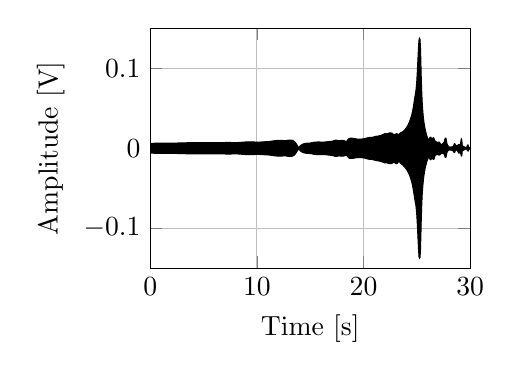
\begin{tikzpicture}

\begin{axis}[%
width=1.6in,
height=1.2in,
at={(0.758in,0.481in)},
scale only axis,
xmin=0,
xmax=30,
xmajorgrids,
ymin=-0.15,
ymax=0.15,
ymajorgrids,
xlabel={Time [s]},
ylabel={Amplitude [V]},
axis background/.style={fill=white}
]
\addplot[fill=black,draw=black,forget plot] plot table[row sep=crcr]{%
2.08333333333333e-05	0.00749385356903076\\
0.0417454218822439	0.00579369068145752\\
0.0834700104311544	0.00580167770385742\\
0.125194598980065	0.00587642192840576\\
0.166919187528975	0.00593435764312744\\
0.208643776077886	0.00599396228790283\\
0.250368364626797	0.0060420036315918\\
0.292092953175707	0.00607657432556152\\
0.333817541724618	0.00612783432006836\\
0.375542130273528	0.00614917278289795\\
0.417266718822439	0.00618958473205566\\
0.458991307371349	0.0061945915222168\\
0.50071589592026	0.00621676445007324\\
0.54244048446917	0.00623643398284912\\
0.584165073018081	0.00624477863311768\\
0.625889661566991	0.00625598430633545\\
0.667614250115902	0.00625300407409668\\
0.709338838664812	0.00626027584075928\\
0.751063427213723	0.00626444816589355\\
0.792788015762633	0.00627720355987549\\
0.834512604311544	0.00626802444458008\\
0.876237192860454	0.00627017021179199\\
0.917961781409365	0.00627803802490234\\
0.959686369958275	0.00628185272216797\\
1.00141095850719	0.00628066062927246\\
1.0431355470561	0.00629818439483643\\
1.08486013560501	0.00629639625549316\\
1.12658472415392	0.00630307197570801\\
1.16830931270283	0.00631487369537354\\
1.21003390125174	0.00632321834564209\\
1.25175848980065	0.00632703304290771\\
1.29348307834956	0.00633490085601807\\
1.33520766689847	0.00633978843688965\\
1.37693225544738	0.0063474178314209\\
1.41865684399629	0.00635361671447754\\
1.4603814325452	0.0063474178314209\\
1.50210602109411	0.00632619857788086\\
1.54383060964302	0.00633561611175537\\
1.58555519819193	0.0063323974609375\\
1.62727978674084	0.00633227825164795\\
1.66900437528975	0.00633740425109863\\
1.71072896383866	0.00631535053253174\\
1.75245355238758	0.00632035732269287\\
1.79417814093649	0.00631523132324219\\
1.8359027294854	0.0063093900680542\\
1.87762731803431	0.00630533695220947\\
1.91935190658322	0.00631821155548096\\
1.96107649513213	0.00632023811340332\\
2.00280108368104	0.00632190704345703\\
2.04452567222995	0.00633811950683594\\
2.08625026077886	0.00633609294891357\\
2.12797484932777	0.0063406229019165\\
2.16969943787668	0.00634121894836426\\
2.21142402642559	0.00634944438934326\\
2.2531486149745	0.00636231899261475\\
2.29487320352341	0.00638401508331299\\
2.33659779207232	0.00638902187347412\\
2.37832238062123	0.00639569759368896\\
2.42004696917014	0.00641250610351563\\
2.46177155771905	0.00643658638000488\\
2.50349614626796	0.00643658638000488\\
2.54522073481687	0.00645923614501953\\
2.58694532336579	0.00647842884063721\\
2.6286699119147	0.00648128986358643\\
2.67039450046361	0.00649750232696533\\
2.71211908901252	0.00650644302368164\\
2.75384367756143	0.00651383399963379\\
2.79556826611034	0.00652897357940674\\
2.83729285465925	0.00654304027557373\\
2.87901744320816	0.00655984878540039\\
2.92074203175707	0.0065767765045166\\
2.96246662030598	0.00659358501434326\\
3.00419120885489	0.0066077709197998\\
3.0459157974038	0.00662326812744141\\
3.08764038595271	0.00664365291595459\\
3.12936497450162	0.00665152072906494\\
3.17108956305053	0.00666582584381104\\
3.21281415159944	0.00668919086456299\\
3.25453874014835	0.00670194625854492\\
3.29626332869726	0.00672006607055664\\
3.33798791724618	0.00670826435089111\\
3.37971250579509	0.00674247741699219\\
3.421437094344	0.00675928592681885\\
3.46316168289291	0.00679123401641846\\
3.50488627144182	0.00679171085357666\\
3.54661085999073	0.00680303573608398\\
3.58833544853964	0.00680971145629883\\
3.63006003708855	0.00682604312896729\\
3.67178462563746	0.00682675838470459\\
3.71350921418637	0.00683438777923584\\
3.75523380273528	0.00683391094207764\\
3.79695839128419	0.00684607028961182\\
3.8386829798331	0.00683021545410156\\
3.88040756838201	0.00682854652404785\\
3.92213215693092	0.0068434476852417\\
3.96385674547983	0.00683057308197021\\
4.00558133402874	0.00684177875518799\\
4.04730592257765	0.0068434476852417\\
4.08903051112656	0.00683856010437012\\
4.13075509967547	0.00683760643005371\\
4.17247968822439	0.00685131549835205\\
4.2142042767733	0.0068504810333252\\
4.25592886532221	0.00685691833496094\\
4.29765345387112	0.00686943531036377\\
4.33937804242003	0.00687718391418457\\
4.38110263096894	0.00688481330871582\\
4.42282721951785	0.00688815116882324\\
4.46455180806676	0.0069044828414917\\
4.50627639661567	0.0069115161895752\\
4.54800098516458	0.00692284107208252\\
4.58972557371349	0.00692355632781982\\
4.6314501622624	0.00694870948791504\\
4.67317475081131	0.00694608688354492\\
4.71489933936022	0.00697565078735352\\
4.75662392790913	0.00697493553161621\\
4.79834851645804	0.00696873664855957\\
4.84007310500695	0.00697898864746094\\
4.88179769355586	0.00699114799499512\\
4.92352228210478	0.00702869892120361\\
4.96524687065368	0.00699985027313232\\
5.0069714592026	0.0070033073425293\\
5.04869604775151	0.00701546669006348\\
5.09042063630042	0.00701582431793213\\
5.13214522484933	0.0070044994354248\\
5.17386981339824	0.00701367855072021\\
5.21559440194715	0.00700652599334717\\
5.25731899049606	0.00701487064361572\\
5.29904357904497	0.0070044994354248\\
5.34076816759388	0.00699400901794434\\
5.38249275614279	0.0070044994354248\\
5.4242173446917	0.00699532032012939\\
5.46594193324061	0.00698482990264893\\
5.50766652178952	0.0069737434387207\\
5.54939111033843	0.00696074962615967\\
5.59111569888734	0.00695204734802246\\
5.63284028743625	0.00692987442016602\\
5.67456487598516	0.00693953037261963\\
5.71628946453407	0.00690567493438721\\
5.75801405308299	0.00688529014587402\\
5.7997386416319	0.00686347484588623\\
5.84146323018081	0.00684857368469238\\
5.88318781872972	0.00684010982513428\\
5.92491240727863	0.00681841373443604\\
5.96663699582754	0.00680434703826904\\
6.00836158437645	0.00681591033935547\\
6.05008617292536	0.00679206848144531\\
6.09181076147427	0.00681543350219727\\
6.13353535002318	0.00681710243225098\\
6.17525993857209	0.00681674480438232\\
6.216984527121	0.00682127475738525\\
6.25870911566991	0.00683438777923584\\
6.30043370421882	0.00684940814971924\\
6.34215829276773	0.00685644149780273\\
6.38388288131664	0.00687861442565918\\
6.42560746986555	0.00686812400817871\\
6.46733205841446	0.00688564777374268\\
6.50905664696338	0.00689232349395752\\
6.55078123551229	0.00691187381744385\\
6.5925058240612	0.00693976879119873\\
6.63423041261011	0.00693285465240479\\
6.67595500115902	0.0069352388381958\\
6.71767958970793	0.0069432258605957\\
6.75940417825684	0.00696563720703125\\
6.80112876680575	0.00698745250701904\\
6.84285335535466	0.00700247287750244\\
6.88457794390357	0.00702583789825439\\
6.92630253245248	0.00702488422393799\\
6.96802712100139	0.00705468654632568\\
7.0097517095503	0.00709474086761475\\
7.05147629809921	0.00712895393371582\\
7.09320088664812	0.00712883472442627\\
7.13492547519703	0.00714349746704102\\
7.17665006374594	0.00718486309051514\\
7.21837465229485	0.0071876049041748\\
7.26009924084376	0.00719738006591797\\
7.30182382939268	0.0072251558303833\\
7.34354841794159	0.00721824169158936\\
7.3852730064905	0.00720977783203125\\
7.42699759503941	0.0072176456451416\\
7.46872218358832	0.00718820095062256\\
7.51044677213723	0.00715470314025879\\
7.55217136068614	0.00714099407196045\\
7.59389594923505	0.00709629058837891\\
7.63562053778396	0.00703322887420654\\
7.67734512633287	0.006980299949646\\
7.71906971488178	0.00693726539611816\\
7.76079430343069	0.00689888000488281\\
7.8025188919796	0.0068976879119873\\
7.84424348052851	0.00685930252075195\\
7.88596806907742	0.00685763359069824\\
7.92769265762633	0.00686526298522949\\
7.96941724617524	0.00687634944915771\\
8.01114183472416	0.00689852237701416\\
8.05286642327307	0.0069270133972168\\
8.09459101182198	0.00695538520812988\\
8.13631560037089	0.00699865818023682\\
8.1780401889198	0.00702321529388428\\
8.21976477746871	0.00706040859222412\\
8.26148936601762	0.00709795951843262\\
8.30321395456653	0.00714755058288574\\
8.34493854311544	0.00716817378997803\\
8.38666313166435	0.00721144676208496\\
8.42838772021326	0.0072711706161499\\
8.47011230876217	0.00730252265930176\\
8.51183689731108	0.00734508037567139\\
8.55356148585999	0.00737583637237549\\
8.5952860744089	0.00743722915649414\\
8.63701066295781	0.00748050212860107\\
8.67873525150672	0.00751698017120361\\
8.72045984005563	0.00755739212036133\\
8.76218442860454	0.00759077072143555\\
8.80390901715345	0.00762379169464111\\
8.84563360570237	0.00767421722412109\\
8.88735819425128	0.00771927833557129\\
8.92908278280018	0.00773894786834717\\
8.9708073713491	0.00777721405029297\\
9.01253195989801	0.00780975818634033\\
9.05425654844692	0.00785017013549805\\
9.09598113699583	0.00786566734313965\\
9.13770572554474	0.00789403915405273\\
9.17943031409365	0.00790119171142578\\
9.22115490264256	0.00791573524475098\\
9.26287949119147	0.00792038440704346\\
9.30460407974038	0.00791454315185547\\
9.34632866828929	0.00792288780212402\\
9.3880532568382	0.00791418552398682\\
9.42977784538711	0.00789248943328857\\
9.47150243393602	0.00790822505950928\\
9.51322702248493	0.00786113739013672\\
9.55495161103384	0.00784194469451904\\
9.59667619958275	0.00783765316009521\\
9.63840078813166	0.00779592990875244\\
9.68012537668058	0.00778317451477051\\
9.72184996522949	0.00776505470275879\\
9.7635745537784	0.0077214241027832\\
9.80529914232731	0.00771212577819824\\
9.84702373087622	0.00768923759460449\\
9.88874831942513	0.00767004489898682\\
9.93047290797404	0.00764584541320801\\
9.97219749652295	0.00761985778808594\\
10.0139220850719	0.00759363174438477\\
10.0556466736208	0.00757205486297607\\
10.0973712621697	0.00758063793182373\\
10.1390958507186	0.00755643844604492\\
10.1808204392675	0.00756394863128662\\
10.2225450278164	0.00758874416351318\\
10.2642696163653	0.00760746002197266\\
10.3059942049142	0.00763463973999023\\
10.3477187934631	0.00768709182739258\\
10.3894433820121	0.0077214241027832\\
10.431167970561	0.00776135921478271\\
10.4728925591099	0.00779759883880615\\
10.5146171476588	0.00784611701965332\\
10.5563417362077	0.00789690017700195\\
10.5980663247566	0.0079195499420166\\
10.6397909133055	0.00797080993652344\\
10.6815155018544	0.00800788402557373\\
10.7232400904033	0.00802457332611084\\
10.7649646789523	0.00804686546325684\\
10.8066892675012	0.00806927680969238\\
10.8484138560501	0.00808560848236084\\
10.890138444599	0.00812733173370361\\
10.9318630331479	0.00815200805664063\\
10.9735876216968	0.00817406177520752\\
11.0153122102457	0.00824487209320068\\
11.0570367987946	0.00827538967132568\\
11.0987613873435	0.00832843780517578\\
11.1404859758924	0.00839519500732422\\
11.1822105644414	0.0084681510925293\\
11.2239351529903	0.00855422019958496\\
11.2656597415392	0.0086212158203125\\
11.3073843300881	0.00867927074432373\\
11.349108918637	0.00874888896942139\\
11.3908335071859	0.00882208347320557\\
11.4325580957348	0.0089038610458374\\
11.4742826842837	0.00899422168731689\\
11.5160072728326	0.00905907154083252\\
11.5577318613816	0.0091407299041748\\
11.5994564499305	0.00920200347900391\\
11.6411810384794	0.00928294658660889\\
11.6829056270283	0.00936365127563477\\
11.7246302155772	0.00943458080291748\\
11.7663548041261	0.00949490070343018\\
11.808079392675	0.00954663753509521\\
11.8498039812239	0.00960981845855713\\
11.8915285697728	0.00966393947601318\\
11.9332531583217	0.00972402095794678\\
11.9749777468707	0.00976741313934326\\
12.0167023354196	0.00980329513549805\\
12.0584269239685	0.00983083248138428\\
12.1001515125174	0.00986802577972412\\
12.1418761010663	0.00987672805786133\\
12.1836006896152	0.00987672805786133\\
12.2253252781641	0.00987434387207031\\
12.267049866713	0.00985038280487061\\
12.3087744552619	0.00976705551147461\\
12.3504990438108	0.00972330570220947\\
12.3922236323598	0.00965023040771484\\
12.4339482209087	0.00957584381103516\\
12.4756728094576	0.0095287561416626\\
12.5173973980065	0.00944745540618896\\
12.5591219865554	0.00940895080566406\\
12.6008465751043	0.00941205024719238\\
12.6425711636532	0.00944828987121582\\
12.6842957522021	0.00948750972747803\\
12.726020340751	0.00955760478973389\\
12.7677449293	0.00966191291809082\\
12.8094695178489	0.00974917411804199\\
12.8511941063978	0.0098346471786499\\
12.8929186949467	0.00993609428405762\\
12.9346432834956	0.0100114345550537\\
12.9763678720445	0.010077953338623\\
13.0180924605934	0.0101412534713745\\
13.0598170491423	0.0101946592330933\\
13.1015416376912	0.0102022886276245\\
13.1432662262401	0.0101913213729858\\
13.1849908147891	0.0101692676544189\\
13.226715403338	0.0101149082183838\\
13.2684399918869	0.0100047588348389\\
13.3101645804358	0.00985205173492432\\
13.3518891689847	0.00965559482574463\\
13.3936137575336	0.00941944122314453\\
13.4353383460825	0.0091102123260498\\
13.4770629346314	0.00872564315795898\\
13.5187875231803	0.00828826427459717\\
13.5605121117293	0.0077366828918457\\
13.6022367002782	0.00710558891296387\\
13.6439612888271	0.00637710094451904\\
13.685685877376	0.0055772066116333\\
13.7274104659249	0.00470268726348877\\
13.7691350544738	0.00378131866455078\\
13.8108596430227	0.00282251834869385\\
13.8525842315716	0.00184452533721924\\
13.8943088201205	0.000988483428955078\\
13.9360334086694	0.00101053714752197\\
13.9777579972184	0.00163733959197998\\
14.0194825857673	0.00229513645172119\\
14.0612071743162	0.00285172462463379\\
14.1029317628651	0.0033571720123291\\
14.144656351414	0.0037921667098999\\
14.1863809399629	0.0041801929473877\\
14.2281055285118	0.00450897216796875\\
14.2698301170607	0.00483500957489014\\
14.3115547056096	0.00506603717803955\\
14.3532792941586	0.00529515743255615\\
14.3950038827075	0.0054936408996582\\
14.4367284712564	0.00565886497497559\\
14.4784530598053	0.00580322742462158\\
14.5201776483542	0.00593674182891846\\
14.5619022369031	0.00600612163543701\\
14.603626825452	0.00609242916107178\\
14.6453514140009	0.00615513324737549\\
14.6870760025498	0.00620019435882568\\
14.7288005910988	0.00623345375061035\\
14.7705251796477	0.00627017021179199\\
14.8122497681966	0.0063014030456543\\
14.8539743567455	0.00632524490356445\\
14.8956989452944	0.00636148452758789\\
14.9374235338433	0.00639736652374268\\
14.9791481223922	0.00643885135650635\\
15.0208727109411	0.00651001930236816\\
15.06259729949	0.00660765171051025\\
15.1043218880389	0.00668370723724365\\
15.1460464765879	0.006827712059021\\
15.1877710651368	0.00696074962615967\\
15.2294956536857	0.00709390640258789\\
15.2712202422346	0.00722610950469971\\
15.3129448307835	0.00731420516967773\\
15.3546694193324	0.007407546043396\\
15.3963940078813	0.00749397277832031\\
15.4381185964302	0.00754451751708984\\
15.4798431849791	0.00758826732635498\\
15.521567773528	0.00765669345855713\\
15.563292362077	0.00769579410552979\\
15.6050169506259	0.00770342350006104\\
15.6467415391748	0.0077279806137085\\
15.6884661277237	0.00774681568145752\\
15.7301907162726	0.00774800777435303\\
15.7719153048215	0.00775599479675293\\
15.8136398933704	0.00774312019348145\\
15.8553644819193	0.00773262977600098\\
15.8970890704682	0.00773715972900391\\
15.9388136590172	0.00769543647766113\\
15.9805382475661	0.00769340991973877\\
16.022262836115	0.00766634941101074\\
16.0639874246639	0.00764882564544678\\
16.1057120132128	0.00762820243835449\\
16.1474366017617	0.00761067867279053\\
16.1891611903106	0.00761198997497559\\
16.2308857788595	0.0076141357421875\\
16.2726103674084	0.00762748718261719\\
16.3143349559573	0.00767076015472412\\
16.3560595445063	0.00773215293884277\\
16.3977841330552	0.00778484344482422\\
16.4395087216041	0.00785326957702637\\
16.481233310153	0.00790536403656006\\
16.5229578987019	0.00796782970428467\\
16.5646824872508	0.00805127620697021\\
16.6064070757997	0.00812697410583496\\
16.6481316643486	0.00818943977355957\\
16.6898562528975	0.00824499130249023\\
16.7315808414465	0.00829720497131348\\
16.7733054299954	0.00836753845214844\\
16.8150300185443	0.00841844081878662\\
16.8567546070932	0.00849032402038574\\
16.8984791956421	0.00852501392364502\\
16.940203784191	0.00859367847442627\\
16.9819283727399	0.0086367130279541\\
17.0236529612888	0.00871849060058594\\
17.0653775498377	0.00880908966064453\\
17.1071021383867	0.00892508029937744\\
17.1488267269356	0.00904440879821777\\
17.1905513154845	0.00922632217407227\\
17.2322759040334	0.00943076610565186\\
17.2740004925823	0.00967895984649658\\
17.3157250811312	0.00985920429229736\\
17.3574496696801	0.00995564460754395\\
17.399174258229	0.00997483730316162\\
17.4408988467779	0.00994551181793213\\
17.4826234353268	0.009865403175354\\
17.5243480238758	0.0097728967666626\\
17.5660726124247	0.00962889194488525\\
17.6077972009736	0.00950288772583008\\
17.6495217895225	0.00936973094940186\\
17.6912463780714	0.00933516025543213\\
17.7329709666203	0.00935065746307373\\
17.7746955551692	0.00944876670837402\\
17.8164201437181	0.00954508781433105\\
17.858144732267	0.0095897912979126\\
17.8998693208159	0.00963819026947021\\
17.9415939093649	0.00966811180114746\\
17.9833184979138	0.00966644287109375\\
18.0250430864627	0.00965023040771484\\
18.0667676750116	0.00961720943450928\\
18.1084922635605	0.00956547260284424\\
18.1502168521094	0.00947082042694092\\
18.1919414406583	0.00928223133087158\\
18.2336660292072	0.00912034511566162\\
18.2753906177561	0.0088578462600708\\
18.3171152063051	0.0086672306060791\\
18.358839794854	0.00849747657775879\\
18.4005643834029	0.00861871242523193\\
18.4422889719518	0.00904262065887451\\
18.4840135605007	0.00969195365905762\\
18.5257381490496	0.0104384422302246\\
18.5674627375985	0.0111484527587891\\
18.6091873261474	0.0116403102874756\\
18.6509119146963	0.0120283365249634\\
18.6926365032453	0.0122295618057251\\
18.7343610917942	0.0123944282531738\\
18.7760856803431	0.0124812126159668\\
18.817810268892	0.012498140335083\\
18.8595348574409	0.0124902725219727\\
18.9012594459898	0.0124739408493042\\
18.9429840345387	0.012393593788147\\
18.9847086230876	0.0123158693313599\\
19.0264332116365	0.0122758150100708\\
19.0681578001854	0.0122194290161133\\
19.1098823887344	0.0121511220932007\\
19.1516069772833	0.012019157409668\\
19.1933315658322	0.011885404586792\\
19.2350561543811	0.0117772817611694\\
19.27678074293	0.0116626024246216\\
19.3185053314789	0.0115736722946167\\
19.3602299200278	0.0114984512329102\\
19.4019545085767	0.0114158391952515\\
19.4436790971256	0.0113530158996582\\
19.4854036856745	0.0113086700439453\\
19.5271282742235	0.0112881660461426\\
19.5688528627724	0.0112816095352173\\
19.6105774513213	0.0112769603729248\\
19.6523020398702	0.0113041400909424\\
19.6940266284191	0.0113296508789063\\
19.735751216968	0.0113605260848999\\
19.7774758055169	0.0113958120346069\\
19.8192003940658	0.0114405155181885\\
19.8609249826147	0.0115052461624146\\
19.9026495711637	0.0115656852722168\\
19.9443741597126	0.0116392374038696\\
19.9860987482615	0.0117192268371582\\
20.0278233368104	0.0118069648742676\\
20.0695479253593	0.0118832588195801\\
20.1112725139082	0.0119979381561279\\
20.1529971024571	0.0121177434921265\\
20.194721691006	0.0122679471969604\\
20.2364462795549	0.0124351978302002\\
20.2781708681038	0.0126054286956787\\
20.3198954566528	0.0127756595611572\\
20.3616200452017	0.01292884349823\\
20.4033446337506	0.0130753517150879\\
20.4450692222995	0.0132129192352295\\
20.4867938108484	0.013319730758667\\
20.5285183993973	0.0133849382400513\\
20.5702429879462	0.013452410697937\\
20.6119675764951	0.0134857892990112\\
20.653692165044	0.0135083198547363\\
20.695416753593	0.0135283470153809\\
20.7371413421419	0.0135420560836792\\
20.7788659306908	0.0135809183120728\\
20.8205905192397	0.0136243104934692\\
20.8623151077886	0.0137261152267456\\
20.9040396963375	0.0138609409332275\\
20.9457642848864	0.014045238494873\\
20.9874888734353	0.0142062902450562\\
21.0292134619842	0.0143966674804688\\
21.0709380505331	0.0145347118377686\\
21.1126626390821	0.0146635770797729\\
21.154387227631	0.0147730112075806\\
21.1961118161799	0.0148556232452393\\
21.2378364047288	0.0149554014205933\\
21.2795609932777	0.0150316953659058\\
21.3212855818266	0.0151089429855347\\
21.3630101703755	0.015178918838501\\
21.4047347589244	0.0152757167816162\\
21.4464593474733	0.0153987407684326\\
21.4881839360223	0.0154969692230225\\
21.5299085245712	0.0156254768371582\\
21.5716331131201	0.0157496929168701\\
21.613357701669	0.0159292221069336\\
21.6550822902179	0.0160981416702271\\
21.6968068787668	0.0163159370422363\\
21.7385314673157	0.0165210962295532\\
21.7802560558646	0.0168144702911377\\
21.8219806444135	0.0170602798461914\\
21.8637052329624	0.0173531770706177\\
21.9054298215114	0.0176330804824829\\
21.9471544100603	0.0178914070129395\\
21.9888789986092	0.0180474519729614\\
22.0306035871581	0.0181217193603516\\
22.072328175707	0.01810622215271\\
22.1140527642559	0.0180014371871948\\
22.1557773528048	0.0178834199905396\\
22.1975019413537	0.0179810523986816\\
22.2392265299026	0.0182150602340698\\
22.2809511184516	0.018438458442688\\
22.3226757070005	0.0186562538146973\\
22.3644002955494	0.0188632011413574\\
22.4061248840983	0.0189707279205322\\
22.4478494726472	0.0190538167953491\\
22.4895740611961	0.0190893411636353\\
22.531298649745	0.0190783739089966\\
22.5730232382939	0.0190154314041138\\
22.6147478268428	0.0189327001571655\\
22.6564724153917	0.018703818321228\\
22.6981970039407	0.0183424949645996\\
22.7399215924896	0.0177360773086548\\
22.7816461810385	0.0173473358154297\\
22.8233707695874	0.0170485973358154\\
22.8650953581363	0.0167936086654663\\
22.9068199466852	0.0168949365615845\\
22.9485445352341	0.0173760652542114\\
22.990269123783	0.0176569223403931\\
23.0319937123319	0.0179094076156616\\
23.0737183008809	0.0180424451828003\\
23.1154428894298	0.018052339553833\\
23.1571674779787	0.0179363489151001\\
23.1988920665276	0.017659068107605\\
23.2406166550765	0.017053484916687\\
23.2823412436254	0.0170373916625977\\
23.3240658321743	0.0173004865646362\\
23.3657904207232	0.0178046226501465\\
23.4075150092721	0.0183619260787964\\
23.449239597821	0.0189418792724609\\
23.49096418637	0.0193721055984497\\
23.5326887749189	0.0196428298950195\\
23.5744133634678	0.0198010206222534\\
23.6161379520167	0.0200726985931396\\
23.6578625405656	0.0203434228897095\\
23.6995871291145	0.0208002328872681\\
23.7413117176634	0.021273136138916\\
23.7830363062123	0.0217666625976563\\
23.8247608947612	0.0223491191864014\\
23.8664854833102	0.0229364633560181\\
23.9082100718591	0.0235723257064819\\
23.949934660408	0.0244051218032837\\
23.9916592489569	0.0251402854919434\\
24.0333838375058	0.0260039567947388\\
24.0751084260547	0.0268300771713257\\
24.1168330146036	0.0277485847473145\\
24.1585576031525	0.0287439823150635\\
24.2002821917014	0.0298217535018921\\
24.2420067802503	0.0309829711914063\\
24.2837313687993	0.0322980880737305\\
24.3254559573482	0.0336868762969971\\
24.3671805458971	0.0352206230163574\\
24.408905134446	0.0368224382400513\\
24.4506297229949	0.0386432409286499\\
24.4923543115438	0.0405960083007813\\
24.5340789000927	0.0426421165466309\\
24.5758034886416	0.0450419187545776\\
24.6175280771905	0.047724723815918\\
24.6592526657395	0.0507631301879883\\
24.7009772542884	0.0541927814483643\\
24.7427018428373	0.057913064956665\\
24.7844264313862	0.0615127086639404\\
24.8261510199351	0.064934253692627\\
24.867875608484	0.068193793296814\\
24.9096001970329	0.0718584060668945\\
24.9513247855818	0.0769494771957397\\
24.9930493741307	0.084394097328186\\
25.0347739626796	0.0938949584960938\\
25.0764985512286	0.105574131011963\\
25.1182231397775	0.116450071334839\\
25.1599477283264	0.128291964530945\\
25.2016723168753	0.13557505607605\\
25.2433969054242	0.137371420860291\\
25.2851214939731	0.136417984962463\\
25.326846082522	0.127503395080566\\
25.3685706710709	0.108487486839294\\
25.4102952596198	0.0855256319046021\\
25.4520198481687	0.0698071718215942\\
25.4937444367177	0.0575932264328003\\
25.5354690252666	0.0487515926361084\\
25.5771936138155	0.0420091152191162\\
25.6189182023644	0.0366709232330322\\
25.6606427909133	0.0323781967163086\\
25.7023673794622	0.0287257432937622\\
25.7440919680111	0.0255154371261597\\
25.78581655656	0.0228915214538574\\
25.8275411451089	0.0203788280487061\\
25.8692657336579	0.0182605981826782\\
25.9109903222068	0.0162765979766846\\
25.9527149107557	0.0145235061645508\\
25.9944394993046	0.0129796266555786\\
26.0361640878535	0.0116792917251587\\
26.0778886764024	0.0108510255813599\\
26.1196132649513	0.0107090473175049\\
26.1613378535002	0.0115089416503906\\
26.2030624420491	0.0128135681152344\\
26.2447870305981	0.0137882232666016\\
26.286511619147	0.0138630867004395\\
26.3282362076959	0.0133175849914551\\
26.3699607962448	0.0115377902984619\\
26.4116853847937	0.0105477571487427\\
26.4534099733426	0.0116112232208252\\
26.4951345618915	0.0127978324890137\\
26.5368591504404	0.013006329536438\\
26.5785837389893	0.0127911567687988\\
26.6203083275383	0.0113941431045532\\
26.6620329160872	0.00994133949279785\\
26.7037575046361	0.00900065898895264\\
26.745482093185	0.00807440280914307\\
26.7872066817339	0.00776731967926025\\
26.8289312702828	0.00786685943603516\\
26.8706558588317	0.00775384902954102\\
26.9123804473806	0.00711297988891602\\
26.9541050359295	0.00681304931640625\\
26.9958296244784	0.00738215446472168\\
27.0375542130274	0.00770378112792969\\
27.0792788015763	0.00770926475524902\\
27.1210033901252	0.00719153881072998\\
27.1627279786741	0.00600016117095947\\
27.204452567223	0.00538229942321777\\
27.2461771557719	0.00485944747924805\\
27.2879017443208	0.00476682186126709\\
27.3296263328697	0.00483024120330811\\
27.3713509214186	0.00507521629333496\\
27.4130755099675	0.00549960136413574\\
27.4548000985165	0.00603604316711426\\
27.4965246870654	0.00652420520782471\\
27.5382492756143	0.00731873512268066\\
27.5799738641632	0.00874698162078857\\
27.6216984527121	0.0109024047851563\\
27.663423041261	0.012520432472229\\
27.7051476298099	0.0126467943191528\\
27.7468722183588	0.0112231969833374\\
27.7885968069077	0.00739848613739014\\
27.8303213954567	0.00537562370300293\\
27.8720459840056	0.0039525032043457\\
27.9137705725545	0.00309288501739502\\
27.9554951611034	0.00234246253967285\\
27.9972197496523	0.00183248519897461\\
28.0389443382012	0.00155806541442871\\
28.0806689267501	0.00140368938446045\\
28.122393515299	0.00123870372772217\\
28.1641181038479	0.00131046772003174\\
28.2058426923968	0.00162017345428467\\
28.2475672809458	0.00169897079467773\\
28.2892918694947	0.00161182880401611\\
28.3310164580436	0.00174915790557861\\
28.3727410465925	0.00210070610046387\\
28.4144656351414	0.00253677368164063\\
28.4561902236903	0.00361108779907227\\
28.4979148122392	0.00531220436096191\\
28.5396394007881	0.00573372840881348\\
28.581363989337	0.00476694107055664\\
28.623088577886	0.00383222103118896\\
28.6648131664349	0.00339996814727783\\
28.7065377549838	0.00311887264251709\\
28.7482623435327	0.00303113460540771\\
28.7899869320816	0.00313305854797363\\
28.8317115206305	0.00360667705535889\\
28.8734361091794	0.00430035591125488\\
28.9151606977283	0.00450372695922852\\
28.9568852862772	0.00431954860687256\\
28.9986098748261	0.00311756134033203\\
29.0403344633751	0.0041656494140625\\
29.082059051924	0.00539898872375488\\
29.1237836404729	0.00856542587280273\\
29.1655082290218	0.011510968208313\\
29.2072328175707	0.0104159116744995\\
29.2489574061196	0.00364077091217041\\
29.2906819946685	0.00311386585235596\\
29.3324065832174	0.00257384777069092\\
29.3741311717663	0.00196397304534912\\
29.4158557603153	0.00168764591217041\\
29.4575803488642	0.00157678127288818\\
29.4993049374131	0.00133764743804932\\
29.541029525962	0.00114858150482178\\
29.5827541145109	0.000946640968322754\\
29.6244787030598	0.000738024711608887\\
29.6662032916087	0.000578761100769043\\
29.7079278801576	0.00254380702972412\\
29.7496524687065	0.00389528274536133\\
29.7913770572554	0.00407397747039795\\
29.8331016458044	0.00197696685791016\\
29.8748262343533	0.00106394290924072\\
29.9165508229022	0.000856161117553711\\
29.9582754114511	0.000536918640136719\\
30	0.000310897827148438\\
}
\closedcycle;
\addplot[fill=black,draw=black,forget plot] plot table[row sep=crcr]{%
2.08333333333333e-05	-0.00700104236602783\\
0.0417454218822439	-0.00586533546447754\\
0.0834700104311544	-0.00591599941253662\\
0.125194598980065	-0.00597560405731201\\
0.166919187528975	-0.00600934028625488\\
0.208643776077886	-0.00608563423156738\\
0.250368364626797	-0.0061333179473877\\
0.292092953175707	-0.00616633892059326\\
0.333817541724618	-0.00620424747467041\\
0.375542130273528	-0.00623416900634766\\
0.417266718822439	-0.00626218318939209\\
0.458991307371349	-0.00628817081451416\\
0.50071589592026	-0.0063023567199707\\
0.54244048446917	-0.00631773471832275\\
0.584165073018081	-0.00631809234619141\\
0.625889661566991	-0.00632476806640625\\
0.667614250115902	-0.0063323974609375\\
0.709338838664812	-0.00635015964508057\\
0.751063427213723	-0.00635278224945068\\
0.792788015762633	-0.00634431838989258\\
0.834512604311544	-0.00638115406036377\\
0.876237192860454	-0.00638151168823242\\
0.917961781409365	-0.0063636302947998\\
0.959686369958275	-0.00636279582977295\\
1.00141095850719	-0.00638449192047119\\
1.0431355470561	-0.00638663768768311\\
1.08486013560501	-0.00640499591827393\\
1.12658472415392	-0.00639533996582031\\
1.16830931270283	-0.00641524791717529\\
1.21003390125174	-0.00641334056854248\\
1.25175848980065	-0.00642001628875732\\
1.29348307834956	-0.00642192363739014\\
1.33520766689847	-0.00643002986907959\\
1.37693225544738	-0.00642740726470947\\
1.41865684399629	-0.00640249252319336\\
1.4603814325452	-0.00643491744995117\\
1.50210602109411	-0.00642955303192139\\
1.54383060964302	-0.00642025470733643\\
1.58555519819193	-0.00642621517181396\\
1.62727978674084	-0.00641453266143799\\
1.66900437528975	-0.00641500949859619\\
1.71072896383866	-0.00641071796417236\\
1.75245355238758	-0.00640082359313965\\
1.79417814093649	-0.00641000270843506\\
1.8359027294854	-0.00641942024230957\\
1.87762731803431	-0.00643205642700195\\
1.91935190658322	-0.00640952587127686\\
1.96107649513213	-0.00639855861663818\\
2.00280108368104	-0.00641703605651855\\
2.04452567222995	-0.00642192363739014\\
2.08625026077886	-0.00642609596252441\\
2.12797484932777	-0.00644028186798096\\
2.16969943787668	-0.00644958019256592\\
2.21142402642559	-0.00646376609802246\\
2.2531486149745	-0.00645744800567627\\
2.29487320352341	-0.00646281242370605\\
2.33659779207232	-0.00647711753845215\\
2.37832238062123	-0.00651836395263672\\
2.42004696917014	-0.006508469581604\\
2.46177155771905	-0.00650954246520996\\
2.50349614626796	-0.00652432441711426\\
2.54522073481687	-0.00656092166900635\\
2.58694532336579	-0.00656425952911377\\
2.6286699119147	-0.0065617561340332\\
2.67039450046361	-0.00657021999359131\\
2.71211908901252	-0.00659680366516113\\
2.75384367756143	-0.00660610198974609\\
2.79556826611034	-0.00662219524383545\\
2.83729285465925	-0.00663149356842041\\
2.87901744320816	-0.00665533542633057\\
2.92074203175707	-0.00666141510009766\\
2.96246662030598	-0.00668776035308838\\
3.00419120885489	-0.00670814514160156\\
3.0459157974038	-0.00671494007110596\\
3.08764038595271	-0.006736159324646\\
3.12936497450162	-0.00674951076507568\\
3.17108956305053	-0.00675570964813232\\
3.21281415159944	-0.00677967071533203\\
3.25453874014835	-0.00681746006011963\\
3.29626332869726	-0.00680828094482422\\
3.33798791724618	-0.00685763359069824\\
3.37971250579509	-0.00683677196502686\\
3.421437094344	-0.0068439245223999\\
3.46316168289291	-0.0068589448928833\\
3.50488627144182	-0.00688552856445313\\
3.54661085999073	-0.00689435005187988\\
3.58833544853964	-0.00691425800323486\\
3.63006003708855	-0.00690722465515137\\
3.67178462563746	-0.00692653656005859\\
3.71350921418637	-0.00692558288574219\\
3.75523380273528	-0.00693893432617188\\
3.79695839128419	-0.0069427490234375\\
3.8386829798331	-0.00694596767425537\\
3.88040756838201	-0.00693023204803467\\
3.92213215693092	-0.00693655014038086\\
3.96385674547983	-0.00693678855895996\\
4.00558133402874	-0.00691890716552734\\
4.04730592257765	-0.00692391395568848\\
4.08903051112656	-0.00697565078735352\\
4.13075509967547	-0.00693845748901367\\
4.17247968822439	-0.00694441795349121\\
4.2142042767733	-0.00693762302398682\\
4.25592886532221	-0.00695562362670898\\
4.29765345387112	-0.00695693492889404\\
4.33937804242003	-0.00696146488189697\\
4.38110263096894	-0.00697410106658936\\
4.42282721951785	-0.00697600841522217\\
4.46455180806676	-0.00698661804199219\\
4.50627639661567	-0.00699365139007568\\
4.54800098516458	-0.00701439380645752\\
4.58972557371349	-0.00701498985290527\\
4.6314501622624	-0.00706160068511963\\
4.67317475081131	-0.00704109668731689\\
4.71489933936022	-0.00705194473266602\\
4.75662392790913	-0.00708127021789551\\
4.79834851645804	-0.00708198547363281\\
4.84007310500695	-0.00709247589111328\\
4.88179769355586	-0.0071028470993042\\
4.92352228210478	-0.00708127021789551\\
4.96524687065368	-0.00708961486816406\\
5.0069714592026	-0.00711381435394287\\
5.04869604775151	-0.00711846351623535\\
5.09042063630042	-0.00711369514465332\\
5.13214522484933	-0.0071178674697876\\
5.17386981339824	-0.0071251392364502\\
5.21559440194715	-0.00710868835449219\\
5.25731899049606	-0.00711417198181152\\
5.29904357904497	-0.00711703300476074\\
5.34076816759388	-0.00711095333099365\\
5.38249275614279	-0.00712096691131592\\
5.4242173446917	-0.00711679458618164\\
5.46594193324061	-0.00708925724029541\\
5.50766652178952	-0.00707530975341797\\
5.54939111033843	-0.00707781314849854\\
5.59111569888734	-0.00706958770751953\\
5.63284028743625	-0.00704407691955566\\
5.67456487598516	-0.00701737403869629\\
5.71628946453407	-0.00702536106109619\\
5.75801405308299	-0.00699901580810547\\
5.7997386416319	-0.0069810152053833\\
5.84146323018081	-0.00696325302124023\\
5.88318781872972	-0.00695526599884033\\
5.92491240727863	-0.0069434642791748\\
5.96663699582754	-0.00694262981414795\\
6.00836158437645	-0.00693976879119873\\
6.05008617292536	-0.00691986083984375\\
6.09181076147427	-0.00692594051361084\\
6.13353535002318	-0.00692093372344971\\
6.17525993857209	-0.00693321228027344\\
6.216984527121	-0.00693976879119873\\
6.25870911566991	-0.00696659088134766\\
6.30043370421882	-0.00698244571685791\\
6.34215829276773	-0.00697767734527588\\
6.38388288131664	-0.00698661804199219\\
6.42560746986555	-0.0070120096206665\\
6.46733205841446	-0.0070120096206665\\
6.50905664696338	-0.00703322887420654\\
6.55078123551229	-0.00704860687255859\\
6.5925058240612	-0.00702023506164551\\
6.63423041261011	-0.00703835487365723\\
6.67595500115902	-0.00705039501190186\\
6.71767958970793	-0.00705540180206299\\
6.75940417825684	-0.00706923007965088\\
6.80112876680575	-0.00707197189331055\\
6.84285335535466	-0.00710380077362061\\
6.88457794390357	-0.00711333751678467\\
6.92630253245248	-0.00713169574737549\\
6.96802712100139	-0.007132887840271\\
7.0097517095503	-0.00714290142059326\\
7.05147629809921	-0.00717353820800781\\
7.09320088664812	-0.0071951150894165\\
7.13492547519703	-0.007224440574646\\
7.17665006374594	-0.00724303722381592\\
7.21837465229485	-0.00727403163909912\\
7.26009924084376	-0.0072789192199707\\
7.30182382939268	-0.00729203224182129\\
7.34354841794159	-0.00731325149536133\\
7.3852730064905	-0.00732207298278809\\
7.42699759503941	-0.00730061531066895\\
7.46872218358832	-0.00727367401123047\\
7.51044677213723	-0.00725102424621582\\
7.55217136068614	-0.00721597671508789\\
7.59389594923505	-0.00717794895172119\\
7.63562053778396	-0.00713169574737549\\
7.67734512633287	-0.0071026086807251\\
7.71906971488178	-0.00705742835998535\\
7.76079430343069	-0.00701916217803955\\
7.8025188919796	-0.00696265697479248\\
7.84424348052851	-0.00694727897644043\\
7.88596806907742	-0.00692427158355713\\
7.92769265762633	-0.00694477558135986\\
7.96941724617524	-0.00694763660430908\\
8.01114183472416	-0.00696742534637451\\
8.05286642327307	-0.00700438022613525\\
8.09459101182198	-0.00702691078186035\\
8.13631560037089	-0.0070720911026001\\
8.1780401889198	-0.00710678100585938\\
8.21976477746871	-0.00713455677032471\\
8.26148936601762	-0.0071793794631958\\
8.30321395456653	-0.00722432136535645\\
8.34493854311544	-0.00728201866149902\\
8.38666313166435	-0.00733113288879395\\
8.42838772021326	-0.00735366344451904\\
8.47011230876217	-0.00739717483520508\\
8.51183689731108	-0.0074317455291748\\
8.55356148585999	-0.00747299194335938\\
8.5952860744089	-0.00752270221710205\\
8.63701066295781	-0.00755190849304199\\
8.67873525150672	-0.00759351253509521\\
8.72045984005563	-0.00764870643615723\\
8.76218442860454	-0.00770199298858643\\
8.80390901715345	-0.0077354907989502\\
8.84563360570237	-0.00774931907653809\\
8.88735819425128	-0.00779211521148682\\
8.92908278280018	-0.0078277587890625\\
8.9708073713491	-0.00787723064422607\\
9.01253195989801	-0.00788784027099609\\
9.05425654844692	-0.00792527198791504\\
9.09598113699583	-0.00794708728790283\\
9.13770572554474	-0.00796234607696533\\
9.17943031409365	-0.00799298286437988\\
9.22115490264256	-0.00799298286437988\\
9.26287949119147	-0.00803208351135254\\
9.30460407974038	-0.00801050662994385\\
9.34632866828929	-0.00799298286437988\\
9.3880532568382	-0.00798630714416504\\
9.42977784538711	-0.00797796249389648\\
9.47150243393602	-0.00795447826385498\\
9.51322702248493	-0.00793743133544922\\
9.55495161103384	-0.00792980194091797\\
9.59667619958275	-0.0079115629196167\\
9.63840078813166	-0.00789284706115723\\
9.68012537668058	-0.00787067413330078\\
9.72184996522949	-0.0078580379486084\\
9.7635745537784	-0.00783014297485352\\
9.80529914232731	-0.0078117847442627\\
9.84702373087622	-0.00777089595794678\\
9.88874831942513	-0.00774955749511719\\
9.93047290797404	-0.0077366828918457\\
9.97219749652295	-0.00769281387329102\\
10.0139220850719	-0.00770032405853271\\
10.0556466736208	-0.00768113136291504\\
10.0973712621697	-0.00765740871429443\\
10.1390958507186	-0.00764620304107666\\
10.1808204392675	-0.00766456127166748\\
10.2225450278164	-0.00767290592193604\\
10.2642696163653	-0.00770699977874756\\
10.3059942049142	-0.00775349140167236\\
10.3477187934631	-0.00777459144592285\\
10.3894433820121	-0.00782191753387451\\
10.431167970561	-0.00786232948303223\\
10.4728925591099	-0.00790190696716309\\
10.5146171476588	-0.00794947147369385\\
10.5563417362077	-0.00799071788787842\\
10.5980663247566	-0.00803661346435547\\
10.6397909133055	-0.00805580615997314\\
10.6815155018544	-0.00807845592498779\\
10.7232400904033	-0.00812423229217529\\
10.7649646789523	-0.00814592838287354\\
10.8066892675012	-0.00816988945007324\\
10.8484138560501	-0.00821030139923096\\
10.890138444599	-0.00821197032928467\\
10.9318630331479	-0.00826525688171387\\
10.9735876216968	-0.00827503204345703\\
11.0153122102457	-0.0083320140838623\\
11.0570367987946	-0.00837600231170654\\
11.0987613873435	-0.00841021537780762\\
11.1404859758924	-0.00847816467285156\\
11.1822105644414	-0.00855040550231934\\
11.2239351529903	-0.00862324237823486\\
11.2656597415392	-0.00869393348693848\\
11.3073843300881	-0.00876319408416748\\
11.349108918637	-0.00884068012237549\\
11.3908335071859	-0.00892031192779541\\
11.4325580957348	-0.00899553298950195\\
11.4742826842837	-0.00906467437744141\\
11.5160072728326	-0.00914371013641357\\
11.5577318613816	-0.00922155380249023\\
11.5994564499305	-0.00928139686584473\\
11.6411810384794	-0.00936257839202881\\
11.6829056270283	-0.00942647457122803\\
11.7246302155772	-0.00948500633239746\\
11.7663548041261	-0.00956261157989502\\
11.808079392675	-0.00963473320007324\\
11.8498039812239	-0.00966012477874756\\
11.8915285697728	-0.00974726676940918\\
11.9332531583217	-0.00978565216064453\\
11.9749777468707	-0.00981950759887695\\
12.0167023354196	-0.00989305973052979\\
12.0584269239685	-0.00990390777587891\\
12.1001515125174	-0.00992751121520996\\
12.1418761010663	-0.00992882251739502\\
12.1836006896152	-0.00993096828460693\\
12.2253252781641	-0.00993132591247559\\
12.267049866713	-0.00991141796112061\\
12.3087744552619	-0.00983965396881104\\
12.3504990438108	-0.00978994369506836\\
12.3922236323598	-0.00968313217163086\\
12.4339482209087	-0.00961101055145264\\
12.4756728094576	-0.00956332683563232\\
12.5173973980065	-0.00949406623840332\\
12.5591219865554	-0.00945484638214111\\
12.6008465751043	-0.00945770740509033\\
12.6425711636532	-0.00949704647064209\\
12.6842957522021	-0.0095444917678833\\
12.726020340751	-0.00961589813232422\\
12.7677449293	-0.00970971584320068\\
12.8094695178489	-0.00977659225463867\\
12.8511941063978	-0.00993132591247559\\
12.8929186949467	-0.00997602939605713\\
12.9346432834956	-0.0100977420806885\\
12.9763678720445	-0.0101566314697266\\
13.0180924605934	-0.0102168321609497\\
13.0598170491423	-0.0102370977401733\\
13.1015416376912	-0.0102627277374268\\
13.1432662262401	-0.0102605819702148\\
13.1849908147891	-0.0102258920669556\\
13.226715403338	-0.0101721286773682\\
13.2684399918869	-0.0100853443145752\\
13.3101645804358	-0.00991141796112061\\
13.3518891689847	-0.00970768928527832\\
13.3936137575336	-0.0094369649887085\\
13.4353383460825	-0.0091477632522583\\
13.4770629346314	-0.00874769687652588\\
13.5187875231803	-0.00827169418334961\\
13.5605121117293	-0.00774753093719482\\
13.6022367002782	-0.0070725679397583\\
13.6439612888271	-0.00634264945983887\\
13.685685877376	-0.00557303428649902\\
13.7274104659249	-0.00468266010284424\\
13.7691350544738	-0.00374627113342285\\
13.8108596430227	-0.00277256965637207\\
13.8525842315716	-0.00178778171539307\\
13.8943088201205	-0.000903606414794922\\
13.9360334086694	-0.00109732151031494\\
13.9777579972184	-0.00177645683288574\\
14.0194825857673	-0.00239205360412598\\
14.0612071743162	-0.00295853614807129\\
14.1029317628651	-0.00349211692810059\\
14.144656351414	-0.0039370059967041\\
14.1863809399629	-0.004302978515625\\
14.2281055285118	-0.00465917587280273\\
14.2698301170607	-0.00494658946990967\\
14.3115547056096	-0.00523078441619873\\
14.3532792941586	-0.00545060634613037\\
14.3950038827075	-0.00563728809356689\\
14.4367284712564	-0.00581169128417969\\
14.4784530598053	-0.00592434406280518\\
14.5201776483542	-0.00603854656219482\\
14.5619022369031	-0.00614619255065918\\
14.603626825452	-0.00621426105499268\\
14.6453514140009	-0.00629508495330811\\
14.6870760025498	-0.00634396076202393\\
14.7288005910988	-0.00639820098876953\\
14.7705251796477	-0.00643074512481689\\
14.8122497681966	-0.00647759437561035\\
14.8539743567455	-0.0065009593963623\\
14.8956989452944	-0.00651967525482178\\
14.9374235338433	-0.00657641887664795\\
14.9791481223922	-0.00661730766296387\\
15.0208727109411	-0.00665640830993652\\
15.06259729949	-0.0067441463470459\\
15.1043218880389	-0.00683927536010742\\
15.1460464765879	-0.00696945190429688\\
15.1877710651368	-0.00709843635559082\\
15.2294956536857	-0.00723099708557129\\
15.2712202422346	-0.0073775053024292\\
15.3129448307835	-0.00749599933624268\\
15.3546694193324	-0.00756645202636719\\
15.3963940078813	-0.0076291561126709\\
15.4381185964302	-0.00770866870880127\\
15.4798431849791	-0.00776588916778564\\
15.521567773528	-0.00780141353607178\\
15.563292362077	-0.00784015655517578\\
15.6050169506259	-0.00786852836608887\\
15.6467415391748	-0.00788617134094238\\
15.6884661277237	-0.0078960657119751\\
15.7301907162726	-0.00790238380432129\\
15.7719153048215	-0.00791895389556885\\
15.8136398933704	-0.00791478157043457\\
15.8553644819193	-0.0078965425491333\\
15.8970890704682	-0.0078890323638916\\
15.9388136590172	-0.00787234306335449\\
15.9805382475661	-0.00787186622619629\\
16.022262836115	-0.00785303115844727\\
16.0639874246639	-0.00780677795410156\\
16.1057120132128	-0.00779342651367188\\
16.1474366017617	-0.00779521465301514\\
16.1891611903106	-0.00780856609344482\\
16.2308857788595	-0.00780689716339111\\
16.2726103674084	-0.00783884525299072\\
16.3143349559573	-0.00787365436553955\\
16.3560595445063	-0.00793659687042236\\
16.3977841330552	-0.00797069072723389\\
16.4395087216041	-0.00803470611572266\\
16.481233310153	-0.00811886787414551\\
16.5229578987019	-0.00819265842437744\\
16.5646824872508	-0.00825834274291992\\
16.6064070757997	-0.00833165645599365\\
16.6481316643486	-0.00837624073028564\\
16.6898562528975	-0.00846719741821289\\
16.7315808414465	-0.00853490829467773\\
16.7733054299954	-0.00857210159301758\\
16.8150300185443	-0.00865054130554199\\
16.8567546070932	-0.0087050199508667\\
16.8984791956421	-0.00876259803771973\\
16.940203784191	-0.00882935523986816\\
16.9819283727399	-0.00888121128082275\\
17.0236529612888	-0.00893664360046387\\
17.0653775498377	-0.00903129577636719\\
17.1071021383867	-0.00913238525390625\\
17.1488267269356	-0.00925207138061523\\
17.1905513154845	-0.00944781303405762\\
17.2322759040334	-0.00966525077819824\\
17.2740004925823	-0.00990176200866699\\
17.3157250811312	-0.0100753307342529\\
17.3574496696801	-0.0101841688156128\\
17.399174258229	-0.0102009773254395\\
17.4408988467779	-0.0101796388626099\\
17.4826234353268	-0.0101015567779541\\
17.5243480238758	-0.00998401641845703\\
17.5660726124247	-0.00984072685241699\\
17.6077972009736	-0.00970554351806641\\
17.6495217895225	-0.00960958003997803\\
17.6912463780714	-0.00957000255584717\\
17.7329709666203	-0.00960838794708252\\
17.7746955551692	-0.00969851016998291\\
17.8164201437181	-0.00977957248687744\\
17.858144732267	-0.00984549522399902\\
17.8998693208159	-0.00989210605621338\\
17.9415939093649	-0.00991296768188477\\
17.9833184979138	-0.00991809368133545\\
18.0250430864627	-0.00989556312561035\\
18.0667676750116	-0.00983786582946777\\
18.1084922635605	-0.00978446006774902\\
18.1502168521094	-0.0096738338470459\\
18.1919414406583	-0.00951778888702393\\
18.2336660292072	-0.00933504104614258\\
18.2753906177561	-0.00913321971893311\\
18.3171152063051	-0.00894129276275635\\
18.358839794854	-0.00878238677978516\\
18.4005643834029	-0.00886201858520508\\
18.4422889719518	-0.00928592681884766\\
18.4840135605007	-0.00993180274963379\\
18.5257381490496	-0.0107002258300781\\
18.5674627375985	-0.0114070177078247\\
18.6091873261474	-0.0119423866271973\\
18.6509119146963	-0.0122295618057251\\
18.6926365032453	-0.012513279914856\\
18.7343610917942	-0.0126503705978394\\
18.7760856803431	-0.0127406120300293\\
18.817810268892	-0.0127830505371094\\
18.8595348574409	-0.0127631425857544\\
18.9012594459898	-0.0127151012420654\\
18.9429840345387	-0.0126211643218994\\
18.9847086230876	-0.0125700235366821\\
19.0264332116365	-0.0125201940536499\\
19.0681578001854	-0.0124548673629761\\
19.1098823887344	-0.0123754739761353\\
19.1516069772833	-0.0122404098510742\\
19.1933315658322	-0.0121179819107056\\
19.2350561543811	-0.0120416879653931\\
19.27678074293	-0.0119369029998779\\
19.3185053314789	-0.0118569135665894\\
19.3602299200278	-0.0117716789245605\\
19.4019545085767	-0.011662483215332\\
19.4436790971256	-0.0116139650344849\\
19.4854036856745	-0.0115795135498047\\
19.5271282742235	-0.0115669965744019\\
19.5688528627724	-0.0115855932235718\\
19.6105774513213	-0.0115777254104614\\
19.6523020398702	-0.0115989446640015\\
19.6940266284191	-0.0116370916366577\\
19.735751216968	-0.011664867401123\\
19.7774758055169	-0.0117090940475464\\
19.8192003940658	-0.0117608308792114\\
19.8609249826147	-0.0118352174758911\\
19.9026495711637	-0.0119103193283081\\
19.9443741597126	-0.0119924545288086\\
19.9860987482615	-0.0120654106140137\\
20.0278233368104	-0.0121363401412964\\
20.0695479253593	-0.0122219324111938\\
20.1112725139082	-0.0123370885848999\\
20.1529971024571	-0.0124459266662598\\
20.194721691006	-0.0126099586486816\\
20.2364462795549	-0.0127689838409424\\
20.2781708681038	-0.012944221496582\\
20.3198954566528	-0.0131044387817383\\
20.3616200452017	-0.0133135318756104\\
20.4033446337506	-0.013464093208313\\
20.4450692222995	-0.0136039257049561\\
20.4867938108484	-0.0137069225311279\\
20.5285183993973	-0.0137710571289063\\
20.5702429879462	-0.0138199329376221\\
20.6119675764951	-0.0138741731643677\\
20.653692165044	-0.0138838291168213\\
20.695416753593	-0.0139110088348389\\
20.7371413421419	-0.0139367580413818\\
20.7788659306908	-0.013996958732605\\
20.8205905192397	-0.014072060585022\\
20.8623151077886	-0.0141732692718506\\
20.9040396963375	-0.0143482685089111\\
20.9457642848864	-0.0145208835601807\\
20.9874888734353	-0.0146999359130859\\
21.0292134619842	-0.0148504972457886\\
21.0709380505331	-0.0150208473205566\\
21.1126626390821	-0.0151451826095581\\
21.154387227631	-0.0152539014816284\\
21.1961118161799	-0.0153449773788452\\
21.2378364047288	-0.0154204368591309\\
21.2795609932777	-0.0155134201049805\\
21.3212855818266	-0.0156024694442749\\
21.3630101703755	-0.0156900882720947\\
21.4047347589244	-0.0157763957977295\\
21.4464593474733	-0.0158889293670654\\
21.4881839360223	-0.0160183906555176\\
21.5299085245712	-0.0161589384078979\\
21.5716331131201	-0.0163154602050781\\
21.613357701669	-0.0164694786071777\\
21.6550822902179	-0.0166647434234619\\
21.6968068787668	-0.0168445110321045\\
21.7385314673157	-0.0170927047729492\\
21.7802560558646	-0.0172708034515381\\
21.8219806444135	-0.0175150632858276\\
21.8637052329624	-0.0177280902862549\\
21.9054298215114	-0.0179343223571777\\
21.9471544100603	-0.0181010961532593\\
21.9888789986092	-0.0182254314422607\\
22.0306035871581	-0.0182375907897949\\
22.072328175707	-0.018206000328064\\
22.1140527642559	-0.018095850944519\\
22.1557773528048	-0.0180206298828125\\
22.1975019413537	-0.0181713104248047\\
22.2392265299026	-0.0184271335601807\\
22.2809511184516	-0.0186953544616699\\
22.3226757070005	-0.018912672996521\\
22.3644002955494	-0.0191589593887329\\
22.4061248840983	-0.0192943811416626\\
22.4478494726472	-0.0193248987197876\\
22.4895740611961	-0.0193195343017578\\
22.531298649745	-0.0193185806274414\\
22.5730232382939	-0.0192511081695557\\
22.6147478268428	-0.0191150903701782\\
22.6564724153917	-0.0188961029052734\\
22.6981970039407	-0.0185633897781372\\
22.7399215924896	-0.0180903673171997\\
22.7816461810385	-0.0177152156829834\\
22.8233707695874	-0.0175611972808838\\
22.8650953581363	-0.0175725221633911\\
22.9068199466852	-0.0178049802780151\\
22.9485445352341	-0.0183752775192261\\
22.990269123783	-0.0186853408813477\\
23.0319937123319	-0.0190421342849731\\
23.0737183008809	-0.0191138982772827\\
23.1154428894298	-0.0190553665161133\\
23.1571674779787	-0.0188769102096558\\
23.1988920665276	-0.0184071063995361\\
23.2406166550765	-0.0174593925476074\\
23.2823412436254	-0.0169633626937866\\
23.3240658321743	-0.0166354179382324\\
23.3657904207232	-0.0169730186462402\\
23.4075150092721	-0.0176547765731812\\
23.449239597821	-0.0183907747268677\\
23.49096418637	-0.0190448760986328\\
23.5326887749189	-0.0195461511611938\\
23.5744133634678	-0.0199412107467651\\
23.6161379520167	-0.0203434228897095\\
23.6578625405656	-0.0207743644714355\\
23.6995871291145	-0.0212763547897339\\
23.7413117176634	-0.0218266248703003\\
23.7830363062123	-0.022449254989624\\
23.8247608947612	-0.0231103897094727\\
23.8664854833102	-0.0237729549407959\\
23.9082100718591	-0.0243896245956421\\
23.949934660408	-0.025164008140564\\
23.9916592489569	-0.0257973670959473\\
24.0333838375058	-0.026525616645813\\
24.0751084260547	-0.0273182392120361\\
24.1168330146036	-0.028288722038269\\
24.1585576031525	-0.0292587280273438\\
24.2002821917014	-0.0303628444671631\\
24.2420067802503	-0.0315853357315063\\
24.2837313687993	-0.0328003168106079\\
24.3254559573482	-0.0341867208480835\\
24.3671805458971	-0.0357458591461182\\
24.408905134446	-0.0373653173446655\\
24.4506297229949	-0.0391743183135986\\
24.4923543115438	-0.0410277843475342\\
24.5340789000927	-0.0431772470474243\\
24.5758034886416	-0.0455392599105835\\
24.6175280771905	-0.048338770866394\\
24.6592526657395	-0.0514264106750488\\
24.7009772542884	-0.0547721385955811\\
24.7427018428373	-0.0583773851394653\\
24.7844264313862	-0.0619864463806152\\
24.8261510199351	-0.0652192831039429\\
24.867875608484	-0.0680805444717407\\
24.9096001970329	-0.0715895891189575\\
24.9513247855818	-0.0767290592193604\\
24.9930493741307	-0.0835990905761719\\
25.0347739626796	-0.0931808948516846\\
25.0764985512286	-0.10465931892395\\
25.1182231397775	-0.116431593894959\\
25.1599477283264	-0.127850890159607\\
25.2016723168753	-0.135683059692383\\
25.2433969054242	-0.137502789497375\\
25.2851214939731	-0.136829257011414\\
25.326846082522	-0.128891110420227\\
25.3685706710709	-0.110212445259094\\
25.4102952596198	-0.0872166156768799\\
25.4520198481687	-0.070671558380127\\
25.4937444367177	-0.0585172176361084\\
25.5354690252666	-0.0500578880310059\\
25.5771936138155	-0.0435303449630737\\
25.6189182023644	-0.0382322072982788\\
25.6606427909133	-0.0339314937591553\\
25.7023673794622	-0.030280590057373\\
25.7440919680111	-0.0270655155181885\\
25.78581655656	-0.0242407321929932\\
25.8275411451089	-0.0218843221664429\\
25.8692657336579	-0.0197430849075317\\
25.9109903222068	-0.0176514387130737\\
25.9527149107557	-0.0158672332763672\\
25.9944394993046	-0.0142406225204468\\
26.0361640878535	-0.0129079818725586\\
26.0778886764024	-0.0116870403289795\\
26.1196132649513	-0.0109869241714478\\
26.1613378535002	-0.0114496946334839\\
26.2030624420491	-0.012880802154541\\
26.2447870305981	-0.0141450166702271\\
26.286511619147	-0.0143531560897827\\
26.3282362076959	-0.0139719247817993\\
26.3699607962448	-0.0123791694641113\\
26.4116853847937	-0.0108746290206909\\
26.4534099733426	-0.0118473768234253\\
26.4951345618915	-0.0133976936340332\\
26.5368591504404	-0.0140365362167358\\
26.5785837389893	-0.013939380645752\\
26.6203083275383	-0.0126149654388428\\
26.6620329160872	-0.0107415914535522\\
26.7037575046361	-0.00921237468719482\\
26.745482093185	-0.00839841365814209\\
26.7872066817339	-0.00812315940856934\\
26.8289312702828	-0.00828778743743896\\
26.8706558588317	-0.00830411911010742\\
26.9123804473806	-0.00782763957977295\\
26.9541050359295	-0.007149338722229\\
26.9958296244784	-0.00746142864227295\\
27.0375542130274	-0.0083082914352417\\
27.0792788015763	-0.00856947898864746\\
27.1210033901252	-0.00843393802642822\\
27.1627279786741	-0.0078272819519043\\
27.204452567223	-0.00741720199584961\\
27.2461771557719	-0.00692653656005859\\
27.2879017443208	-0.00661814212799072\\
27.3296263328697	-0.00642073154449463\\
27.3713509214186	-0.00631809234619141\\
27.4130755099675	-0.00635647773742676\\
27.4548000985165	-0.00659608840942383\\
27.4965246870654	-0.00683295726776123\\
27.5382492756143	-0.00733041763305664\\
27.5799738641632	-0.00845849514007568\\
27.6216984527121	-0.0100034475326538\\
27.663423041261	-0.0112991333007813\\
27.7051476298099	-0.0113341808319092\\
27.7468722183588	-0.0100919008255005\\
27.7885968069077	-0.00659024715423584\\
27.8303213954567	-0.00476396083831787\\
27.8720459840056	-0.00387775897979736\\
27.9137705725545	-0.0032498836517334\\
27.9554951611034	-0.00279760360717773\\
27.9972197496523	-0.00246703624725342\\
28.0389443382012	-0.00212502479553223\\
28.0806689267501	-0.00186002254486084\\
28.122393515299	-0.00188124179840088\\
28.1641181038479	-0.00229358673095703\\
28.2058426923968	-0.002494215965271\\
28.2475672809458	-0.00231277942657471\\
28.2892918694947	-0.00244450569152832\\
28.3310164580436	-0.00275528430938721\\
28.3727410465925	-0.00312244892120361\\
28.4144656351414	-0.00383174419403076\\
28.4561902236903	-0.00467133522033691\\
28.4979148122392	-0.00538063049316406\\
28.5396394007881	-0.00525295734405518\\
28.581363989337	-0.00360226631164551\\
28.623088577886	-0.00249123573303223\\
28.6648131664349	-0.00228774547576904\\
28.7065377549838	-0.00232863426208496\\
28.7482623435327	-0.00244617462158203\\
28.7899869320816	-0.00303876399993896\\
28.8317115206305	-0.00371408462524414\\
28.8734361091794	-0.00466454029083252\\
28.9151606977283	-0.00596809387207031\\
28.9568852862772	-0.00609028339385986\\
28.9986098748261	-0.00471508502960205\\
29.0403344633751	-0.00482821464538574\\
29.082059051924	-0.00568509101867676\\
29.1237836404729	-0.00717794895172119\\
29.1655082290218	-0.0096893310546875\\
29.2072328175707	-0.00945603847503662\\
29.2489574061196	-0.00364315509796143\\
29.2906819946685	-0.00262188911437988\\
29.3324065832174	-0.00270700454711914\\
29.3741311717663	-0.0025324821472168\\
29.4158557603153	-0.00185918807983398\\
29.4575803488642	-0.00171053409576416\\
29.4993049374131	-0.00135767459869385\\
29.541029525962	-0.00111198425292969\\
29.5827541145109	-0.000892758369445801\\
29.6244787030598	-0.00065302848815918\\
29.6662032916087	-0.000777244567871094\\
29.7079278801576	-0.00211238861083984\\
29.7496524687065	-0.00314760208129883\\
29.7913770572554	-0.00347006320953369\\
29.8331016458044	-0.00233721733093262\\
29.8748262343533	-0.00166881084442139\\
29.9165508229022	-0.000946760177612305\\
29.9582754114511	-0.000213503837585449\\
30	-0.000554800033569336\\
}
\closedcycle;
\end{axis}
\end{tikzpicture}%
%\caption{Accelerometer på driver - Måling 10}
%\end{subfigure}
%\begin{subfigure}[t]{0.45\textwidth}
%\centering
%%\includegraphics[width=\textwidth]{raw_driver19}
%% This file was created by matlab2tikz.
%
%The latest updates can be retrieved from
%  http://www.mathworks.com/matlabcentral/fileexchange/22022-matlab2tikz-matlab2tikz
%where you can also make suggestions and rate matlab2tikz.
%
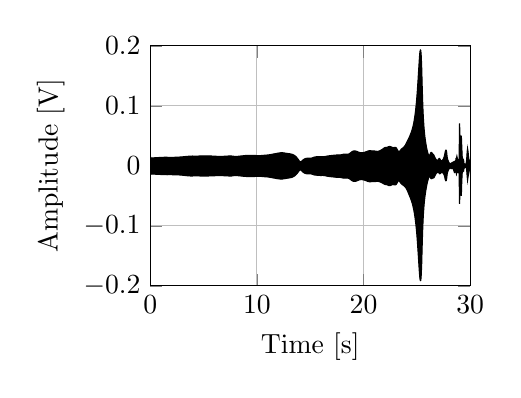
\begin{tikzpicture}

\begin{axis}[%
width=1.6in,
height=1.2in,
at={(0.758in,0.481in)},
scale only axis,
xmin=0,
xmax=30,
xmajorgrids,
ymin=-0.2,
ymax=0.2,
ymajorgrids,
xlabel={Time [s]},
ylabel={Amplitude [V]},
axis background/.style={fill=white}
]
\addplot[fill=black,draw=black,forget plot] plot table[row sep=crcr]{%
2.08333333333333e-05	0.0174441337585449\\
0.0417454218822439	0.0131838321685791\\
0.0834700104311544	0.0131036043167114\\
0.125194598980065	0.0131006240844727\\
0.166919187528975	0.0131523609161377\\
0.208643776077886	0.0131937265396118\\
0.250368364626797	0.013242244720459\\
0.292092953175707	0.0132843255996704\\
0.333817541724618	0.0133000612258911\\
0.375542130273528	0.0133227109909058\\
0.417266718822439	0.0133814811706543\\
0.458991307371349	0.0134208202362061\\
0.50071589592026	0.0134570598602295\\
0.54244048446917	0.0134916305541992\\
0.584165073018081	0.0135313272476196\\
0.625889661566991	0.0135787725448608\\
0.667614250115902	0.0136535167694092\\
0.709338838664812	0.0136919021606445\\
0.751063427213723	0.0137407779693604\\
0.792788015762633	0.01378333568573\\
0.834512604311544	0.0138405561447144\\
0.876237192860454	0.0138554573059082\\
0.917961781409365	0.0138992071151733\\
0.959686369958275	0.0139317512512207\\
1.00141095850719	0.0139665603637695\\
1.0431355470561	0.0140010118484497\\
1.08486013560501	0.0140565633773804\\
1.12658472415392	0.0140770673751831\\
1.16830931270283	0.0141662359237671\\
1.21003390125174	0.0141417980194092\\
1.25175848980065	0.014143705368042\\
1.29348307834956	0.0142022371292114\\
1.33520766689847	0.014235258102417\\
1.37693225544738	0.0142310857772827\\
1.41865684399629	0.0142514705657959\\
1.4603814325452	0.0142501592636108\\
1.50210602109411	0.0142426490783691\\
1.54383060964302	0.0142196416854858\\
1.58555519819193	0.0141897201538086\\
1.62727978674084	0.0141717195510864\\
1.66900437528975	0.0141562223434448\\
1.71072896383866	0.0141338109970093\\
1.75245355238758	0.0141158103942871\\
1.79417814093649	0.0141069889068604\\
1.8359027294854	0.014079213142395\\
1.87762731803431	0.0140920877456665\\
1.91935190658322	0.0140824317932129\\
1.96107649513213	0.014080286026001\\
2.00280108368104	0.0140819549560547\\
2.04452567222995	0.0140804052352905\\
2.08625026077886	0.0140907764434814\\
2.12797484932777	0.0141453742980957\\
2.16969943787668	0.0141212940216064\\
2.21142402642559	0.014117956161499\\
2.2531486149745	0.0141592025756836\\
2.29487320352341	0.0141942501068115\\
2.33659779207232	0.0142147541046143\\
2.37832238062123	0.014255166053772\\
2.42004696917014	0.0142718553543091\\
2.46177155771905	0.0143097639083862\\
2.50349614626796	0.0143415927886963\\
2.54522073481687	0.0143803358078003\\
2.58694532336579	0.0144282579421997\\
2.6286699119147	0.014466404914856\\
2.67039450046361	0.0145164728164673\\
2.71211908901252	0.0145268440246582\\
2.75384367756143	0.0145998001098633\\
2.79556826611034	0.014657735824585\\
2.83729285465925	0.0147078037261963\\
2.87901744320816	0.014757513999939\\
2.92074203175707	0.0148080587387085\\
2.96246662030598	0.0148706436157227\\
3.00419120885489	0.0149272680282593\\
3.0459157974038	0.0149846076965332\\
3.08764038595271	0.0150657892227173\\
3.12936497450162	0.0151398181915283\\
3.17108956305053	0.0152368545532227\\
3.21281415159944	0.0153077840805054\\
3.25453874014835	0.0153566598892212\\
3.29626332869726	0.0154335498809814\\
3.33798791724618	0.0155411958694458\\
3.37971250579509	0.0155764818191528\\
3.421437094344	0.0156253576278687\\
3.46316168289291	0.0156955718994141\\
3.50488627144182	0.015771746635437\\
3.54661085999073	0.0158456563949585\\
3.58833544853964	0.0159142017364502\\
3.63006003708855	0.0159842967987061\\
3.67178462563746	0.0160502195358276\\
3.71350921418637	0.0160926580429077\\
3.75523380273528	0.0161477327346802\\
3.79695839128419	0.01618492603302\\
3.8386829798331	0.0162196159362793\\
3.88040756838201	0.0162382125854492\\
3.92213215693092	0.0162550210952759\\
3.96385674547983	0.0162825584411621\\
4.00558133402874	0.0162662267684937\\
4.04730592257765	0.0162646770477295\\
4.08903051112656	0.0162562131881714\\
4.13075509967547	0.0162286758422852\\
4.17247968822439	0.0162371397018433\\
4.2142042767733	0.0162320137023926\\
4.25592886532221	0.0162011384963989\\
4.29765345387112	0.0161941051483154\\
4.33937804242003	0.0161887407302856\\
4.38110263096894	0.0161789655685425\\
4.42282721951785	0.0162254571914673\\
4.46455180806676	0.0162070989608765\\
4.50627639661567	0.0162445306777954\\
4.54800098516458	0.0162758827209473\\
4.58972557371349	0.0163146257400513\\
4.6314501622624	0.0163501501083374\\
4.67317475081131	0.0163940191268921\\
4.71489933936022	0.0164343118667603\\
4.75662392790913	0.0164703130722046\\
4.79834851645804	0.0165045261383057\\
4.84007310500695	0.0165075063705444\\
4.88179769355586	0.0165128707885742\\
4.92352228210478	0.0165145397186279\\
4.96524687065368	0.0165392160415649\\
5.0069714592026	0.0165344476699829\\
5.04869604775151	0.0165383815765381\\
5.09042063630042	0.0165327787399292\\
5.13214522484933	0.0165436267852783\\
5.17386981339824	0.0165482759475708\\
5.21559440194715	0.0165524482727051\\
5.25731899049606	0.0165770053863525\\
5.29904357904497	0.0165486335754395\\
5.34076816759388	0.016539454460144\\
5.38249275614279	0.0165292024612427\\
5.4242173446917	0.0165091753005981\\
5.46594193324061	0.01650071144104\\
5.50766652178952	0.0164941549301147\\
5.54939111033843	0.0164557695388794\\
5.59111569888734	0.0164422988891602\\
5.63284028743625	0.0164107084274292\\
5.67456487598516	0.0163847208023071\\
5.71628946453407	0.0163488388061523\\
5.75801405308299	0.0162984132766724\\
5.7997386416319	0.016254186630249\\
5.84146323018081	0.0161999464035034\\
5.88318781872972	0.0161627531051636\\
5.92491240727863	0.016115665435791\\
5.96663699582754	0.0160861015319824\\
6.00836158437645	0.0160255432128906\\
6.05008617292536	0.0159963369369507\\
6.09181076147427	0.0159608125686646\\
6.13353535002318	0.015892505645752\\
6.17525993857209	0.0158644914627075\\
6.216984527121	0.0158439874649048\\
6.25870911566991	0.0158376693725586\\
6.30043370421882	0.015795111656189\\
6.34215829276773	0.0157642364501953\\
6.38388288131664	0.0157539844512939\\
6.42560746986555	0.0157680511474609\\
6.46733205841446	0.0157626867294312\\
6.50905664696338	0.0157822370529175\\
6.55078123551229	0.0157889127731323\\
6.5925058240612	0.01578688621521\\
6.63423041261011	0.015788197517395\\
6.67595500115902	0.0158027410507202\\
6.71767958970793	0.0158090591430664\\
6.75940417825684	0.0158181190490723\\
6.80112876680575	0.0158118009567261\\
6.84285335535466	0.0158218145370483\\
6.88457794390357	0.0158369541168213\\
6.92630253245248	0.0158761739730835\\
6.96802712100139	0.0158882141113281\\
7.0097517095503	0.0159152746200562\\
7.05147629809921	0.015964150428772\\
7.09320088664812	0.0159767866134644\\
7.13492547519703	0.0160250663757324\\
7.17665006374594	0.0161073207855225\\
7.21837465229485	0.0161528587341309\\
7.26009924084376	0.0162261724472046\\
7.30182382939268	0.0163071155548096\\
7.34354841794159	0.0163383483886719\\
7.3852730064905	0.016379714012146\\
7.42699759503941	0.0164109468460083\\
7.46872218358832	0.0164202451705933\\
7.51044677213723	0.01641845703125\\
7.55217136068614	0.0163893699645996\\
7.59389594923505	0.0163551568984985\\
7.63562053778396	0.016291618347168\\
7.67734512633287	0.0162198543548584\\
7.71906971488178	0.0161285400390625\\
7.76079430343069	0.016048789024353\\
7.8025188919796	0.0159471035003662\\
7.84424348052851	0.0158181190490723\\
7.88596806907742	0.0157514810562134\\
7.92769265762633	0.0156846046447754\\
7.96941724617524	0.0156430006027222\\
8.01114183472416	0.0156441926956177\\
8.05286642327307	0.015630841255188\\
8.09459101182198	0.0156680345535278\\
8.13631560037089	0.015711784362793\\
8.1780401889198	0.0157798528671265\\
8.21976477746871	0.0158299207687378\\
8.26148936601762	0.0159074068069458\\
8.30321395456653	0.0159891843795776\\
8.34493854311544	0.01605224609375\\
8.38666313166435	0.0161564350128174\\
8.42838772021326	0.0162137746810913\\
8.47011230876217	0.0163058042526245\\
8.51183689731108	0.0163658857345581\\
8.55356148585999	0.0164523124694824\\
8.5952860744089	0.0164806842803955\\
8.63701066295781	0.0166155099868774\\
8.67873525150672	0.0166575908660889\\
8.72045984005563	0.0167548656463623\\
8.76218442860454	0.016825795173645\\
8.80390901715345	0.0169020891189575\\
8.84563360570237	0.0169821977615356\\
8.88735819425128	0.0170701742172241\\
8.92908278280018	0.0171375274658203\\
8.9708073713491	0.0171587467193604\\
9.01253195989801	0.017237663269043\\
9.05425654844692	0.0172935724258423\\
9.09598113699583	0.0173218250274658\\
9.13770572554474	0.0173497200012207\\
9.17943031409365	0.0173822641372681\\
9.22115490264256	0.0174020528793335\\
9.26287949119147	0.0174028873443604\\
9.30460407974038	0.0174020528793335\\
9.34632866828929	0.017397403717041\\
9.3880532568382	0.017382025718689\\
9.42977784538711	0.0173323154449463\\
9.47150243393602	0.0173298120498657\\
9.51322702248493	0.0173071622848511\\
9.55495161103384	0.0172981023788452\\
9.59667619958275	0.0172533988952637\\
9.63840078813166	0.0172268152236938\\
9.68012537668058	0.0172126293182373\\
9.72184996522949	0.0172011852264404\\
9.7635745537784	0.0171804428100586\\
9.80529914232731	0.0171520709991455\\
9.84702373087622	0.0171386003494263\\
9.88874831942513	0.0171166658401489\\
9.93047290797404	0.0170993804931641\\
9.97219749652295	0.0170501470565796\\
10.0139220850719	0.0170356035232544\\
10.0556466736208	0.0170102119445801\\
10.0973712621697	0.0169705152511597\\
10.1390958507186	0.0169491767883301\\
10.1808204392675	0.0169264078140259\\
10.2225450278164	0.0169349908828735\\
10.2642696163653	0.016948938369751\\
10.3059942049142	0.0169826745986938\\
10.3477187934631	0.0170327425003052\\
10.3894433820121	0.0170915126800537\\
10.431167970561	0.0171574354171753\\
10.4728925591099	0.0172317028045654\\
10.5146171476588	0.0172722339630127\\
10.5563417362077	0.0173627138137817\\
10.5980663247566	0.0174278020858765\\
10.6397909133055	0.0175130367279053\\
10.6815155018544	0.0175483226776123\\
10.7232400904033	0.0176342725753784\\
10.7649646789523	0.0176903009414673\\
10.8066892675012	0.0177403688430786\\
10.8484138560501	0.0177834033966064\\
10.890138444599	0.0178585052490234\\
10.9318630331479	0.0179126262664795\\
10.9735876216968	0.0179930925369263\\
11.0153122102457	0.0180377960205078\\
11.0570367987946	0.0181233882904053\\
11.0987613873435	0.0181983709335327\\
11.1404859758924	0.0183128118515015\\
11.1822105644414	0.0184154510498047\\
11.2239351529903	0.0185511112213135\\
11.2656597415392	0.0186648368835449\\
11.3073843300881	0.0188018083572388\\
11.349108918637	0.0189625024795532\\
11.3908335071859	0.0190943479537964\\
11.4325580957348	0.0192328691482544\\
11.4742826842837	0.0194246768951416\\
11.5160072728326	0.0195508003234863\\
11.5577318613816	0.019692063331604\\
11.5994564499305	0.0198198556900024\\
11.6411810384794	0.0199755430221558\\
11.6829056270283	0.0201060771942139\\
11.7246302155772	0.0202442407608032\\
11.7663548041261	0.0203926563262939\\
11.808079392675	0.0205307006835938\\
11.8498039812239	0.0206559896469116\\
11.8915285697728	0.0208258628845215\\
11.9332531583217	0.0209463834762573\\
11.9749777468707	0.0210902690887451\\
12.0167023354196	0.0212063789367676\\
12.0584269239685	0.0213172435760498\\
12.1001515125174	0.0214052200317383\\
12.1418761010663	0.0215300321578979\\
12.1836006896152	0.0216346979141235\\
12.2253252781641	0.0217214822769165\\
12.267049866713	0.0217512845993042\\
12.3087744552619	0.0217386484146118\\
12.3504990438108	0.0217629671096802\\
12.3922236323598	0.0217190980911255\\
12.4339482209087	0.0217164754867554\\
12.4756728094576	0.0216211080551147\\
12.5173973980065	0.0215216875076294\\
12.5591219865554	0.0214111804962158\\
12.6008465751043	0.0212830305099487\\
12.6425711636532	0.0211762189865112\\
12.6842957522021	0.0210355520248413\\
12.726020340751	0.0209170579910278\\
12.7677449293	0.0208185911178589\\
12.8094695178489	0.0207177400588989\\
12.8511941063978	0.0206308364868164\\
12.8929186949467	0.0205261707305908\\
12.9346432834956	0.0204188823699951\\
12.9763678720445	0.0203160047531128\\
13.0180924605934	0.0202019214630127\\
13.0598170491423	0.020089864730835\\
13.1015416376912	0.0199722051620483\\
13.1432662262401	0.0198445320129395\\
13.1849908147891	0.0197038650512695\\
13.226715403338	0.0195189714431763\\
13.2684399918869	0.0193073749542236\\
13.3101645804358	0.0190596580505371\\
13.3518891689847	0.0188181400299072\\
13.3936137575336	0.0185122489929199\\
13.4353383460825	0.0181918144226074\\
13.4770629346314	0.0177853107452393\\
13.5187875231803	0.0173110961914063\\
13.5605121117293	0.0167787075042725\\
13.6022367002782	0.0161740779876709\\
13.6439612888271	0.0155293941497803\\
13.685685877376	0.0147796869277954\\
13.7274104659249	0.0139639377593994\\
13.7691350544738	0.0130655765533447\\
13.8108596430227	0.0121190547943115\\
13.8525842315716	0.011111855506897\\
13.8943088201205	0.0100915431976318\\
13.9360334086694	0.00906765460968018\\
13.9777579972184	0.0081101655960083\\
14.0194825857673	0.00735759735107422\\
14.0612071743162	0.00674760341644287\\
14.1029317628651	0.00652647018432617\\
14.144656351414	0.00688815116882324\\
14.1863809399629	0.00745463371276855\\
14.2281055285118	0.00815272331237793\\
14.2698301170607	0.00885546207427979\\
14.3115547056096	0.00954830646514893\\
14.3532792941586	0.0101321935653687\\
14.3950038827075	0.0106920003890991\\
14.4367284712564	0.0111517906188965\\
14.4784530598053	0.0115351676940918\\
14.5201776483542	0.0118722915649414\\
14.5619022369031	0.0121043920516968\\
14.603626825452	0.0123043060302734\\
14.6453514140009	0.0124328136444092\\
14.6870760025498	0.0125536918640137\\
14.7288005910988	0.0126279592514038\\
14.7705251796477	0.0126522779464722\\
14.8122497681966	0.0126771926879883\\
14.8539743567455	0.0126643180847168\\
14.8956989452944	0.0126442909240723\\
14.9374235338433	0.0126314163208008\\
14.9791481223922	0.0126005411148071\\
15.0208727109411	0.0125870704650879\\
15.06259729949	0.0126197338104248\\
15.1043218880389	0.0127360820770264\\
15.1460464765879	0.0129470825195313\\
15.1877710651368	0.0131411552429199\\
15.2294956536857	0.0134528875350952\\
15.2712202422346	0.0137631893157959\\
15.3129448307835	0.014081597328186\\
15.3546694193324	0.0143324136734009\\
15.3963940078813	0.0145440101623535\\
15.4381185964302	0.0147069692611694\\
15.4798431849791	0.014826774597168\\
15.521567773528	0.0149147510528564\\
15.563292362077	0.0150187015533447\\
15.6050169506259	0.0150867700576782\\
15.6467415391748	0.0151418447494507\\
15.6884661277237	0.0152006149291992\\
15.7301907162726	0.0152875185012817\\
15.7719153048215	0.015317440032959\\
15.8136398933704	0.0153570175170898\\
15.8553644819193	0.0153845548629761\\
15.8970890704682	0.0154201984405518\\
15.9388136590172	0.0154287815093994\\
15.9805382475661	0.0154200792312622\\
16.022262836115	0.0154227018356323\\
16.0639874246639	0.0153900384902954\\
16.1057120132128	0.0153504610061646\\
16.1474366017617	0.0152820348739624\\
16.1891611903106	0.0152740478515625\\
16.2308857788595	0.0152736902236938\\
16.2726103674084	0.0152853727340698\\
16.3143349559573	0.0153579711914063\\
16.3560595445063	0.0154263973236084\\
16.3977841330552	0.0155422687530518\\
16.4395087216041	0.0156645774841309\\
16.481233310153	0.015790581703186\\
16.5229578987019	0.0159449577331543\\
16.5646824872508	0.0161056518554688\\
16.6064070757997	0.0162507295608521\\
16.6481316643486	0.0163685083389282\\
16.6898562528975	0.0164653062820435\\
16.7315808414465	0.0165603160858154\\
16.7733054299954	0.0167076587677002\\
16.8150300185443	0.0167895555496216\\
16.8567546070932	0.0168788433074951\\
16.8984791956421	0.0169848203659058\\
16.940203784191	0.017051100730896\\
16.9819283727399	0.017139196395874\\
17.0236529612888	0.0172312259674072\\
17.0653775498377	0.0173563957214355\\
17.1071021383867	0.0174448490142822\\
17.1488267269356	0.0174803733825684\\
17.1905513154845	0.0175639390945435\\
17.2322759040334	0.0176322460174561\\
17.2740004925823	0.0177028179168701\\
17.3157250811312	0.017791748046875\\
17.3574496696801	0.0178496837615967\\
17.399174258229	0.0178979635238647\\
17.4408988467779	0.017961859703064\\
17.4826234353268	0.018022894859314\\
17.5243480238758	0.018062949180603\\
17.5660726124247	0.01810622215271\\
17.6077972009736	0.0180763006210327\\
17.6495217895225	0.0180815458297729\\
17.6912463780714	0.0180732011795044\\
17.7329709666203	0.0180991888046265\\
17.7746955551692	0.0181357860565186\\
17.8164201437181	0.018202543258667\\
17.858144732267	0.0183231830596924\\
17.8998693208159	0.0184512138366699\\
17.9415939093649	0.0185703039169312\\
17.9833184979138	0.0187492370605469\\
18.0250430864627	0.0189353227615356\\
18.0667676750116	0.0190675258636475\\
18.1084922635605	0.0192264318466187\\
18.1502168521094	0.0192973613739014\\
18.1919414406583	0.0193362236022949\\
18.2336660292072	0.0193533897399902\\
18.2753906177561	0.0193248987197876\\
18.3171152063051	0.0193346738815308\\
18.358839794854	0.0192720890045166\\
18.4005643834029	0.0192611217498779\\
18.4422889719518	0.0192636251449585\\
18.4840135605007	0.0192739963531494\\
18.5257381490496	0.0192903280258179\\
18.5674627375985	0.0194275379180908\\
18.6091873261474	0.0196996927261353\\
18.6509119146963	0.0200306177139282\\
18.6926365032453	0.0204979181289673\\
18.7343610917942	0.02104651927948\\
18.7760856803431	0.0216186046600342\\
18.817810268892	0.0222443342208862\\
18.8595348574409	0.0227910280227661\\
18.9012594459898	0.0233092308044434\\
18.9429840345387	0.023730993270874\\
18.9847086230876	0.0240856409072876\\
19.0264332116365	0.0244448184967041\\
19.0681578001854	0.0246785879135132\\
19.1098823887344	0.0248157978057861\\
19.1516069772833	0.0248291492462158\\
19.1933315658322	0.0247887372970581\\
19.2350561543811	0.0246955156326294\\
19.27678074293	0.0245308876037598\\
19.3185053314789	0.0243546962738037\\
19.3602299200278	0.0240871906280518\\
19.4019545085767	0.0237839221954346\\
19.4436790971256	0.0234526395797729\\
19.4854036856745	0.0231184959411621\\
19.5271282742235	0.022815465927124\\
19.5688528627724	0.0225284099578857\\
19.6105774513213	0.0223060846328735\\
19.6523020398702	0.0221070051193237\\
19.6940266284191	0.0219635963439941\\
19.735751216968	0.0218530893325806\\
19.7774758055169	0.0217581987380981\\
19.8192003940658	0.0217596292495728\\
19.8609249826147	0.0217828750610352\\
19.9026495711637	0.0218667984008789\\
19.9443741597126	0.0219509601593018\\
19.9860987482615	0.0220874547958374\\
20.0278233368104	0.0222543478012085\\
20.0695479253593	0.0224721431732178\\
20.1112725139082	0.0226690769195557\\
20.1529971024571	0.0229157209396362\\
20.194721691006	0.0231697559356689\\
20.2364462795549	0.0234352350234985\\
20.2781708681038	0.0237188339233398\\
20.3198954566528	0.0240160226821899\\
20.3616200452017	0.0242964029312134\\
20.4033446337506	0.024566650390625\\
20.4450692222995	0.0247782468795776\\
20.4867938108484	0.0249801874160767\\
20.5285183993973	0.025060772895813\\
20.5702429879462	0.0250948667526245\\
20.6119675764951	0.0251015424728394\\
20.653692165044	0.025084376335144\\
20.695416753593	0.0250260829925537\\
20.7371413421419	0.0249568223953247\\
20.7788659306908	0.0249083042144775\\
20.8205905192397	0.0248545408248901\\
20.8623151077886	0.0248538255691528\\
20.9040396963375	0.0248321294784546\\
20.9457642848864	0.0248123407363892\\
20.9874888734353	0.0247715711593628\\
21.0292134619842	0.0246872901916504\\
21.0709380505331	0.0245916843414307\\
21.1126626390821	0.0244895219802856\\
21.154387227631	0.0243560075759888\\
21.1961118161799	0.0242257118225098\\
21.2378364047288	0.0241231918334961\\
21.2795609932777	0.0240743160247803\\
21.3212855818266	0.0240955352783203\\
21.3630101703755	0.0242211818695068\\
21.4047347589244	0.0243576765060425\\
21.4464593474733	0.0245411396026611\\
21.4881839360223	0.0248323678970337\\
21.5299085245712	0.0251299142837524\\
21.5716331131201	0.0254895687103271\\
21.613357701669	0.0259164571762085\\
21.6550822902179	0.0263410806655884\\
21.6968068787668	0.0268235206604004\\
21.7385314673157	0.0273033380508423\\
21.7802560558646	0.0278036594390869\\
21.8219806444135	0.0282833576202393\\
21.8637052329624	0.0288461446762085\\
21.9054298215114	0.0293409824371338\\
21.9471544100603	0.0298067331314087\\
21.9888789986092	0.0302213430404663\\
22.0306035871581	0.0305540561676025\\
22.072328175707	0.0307530164718628\\
22.1140527642559	0.0307987928390503\\
22.1557773528048	0.030825138092041\\
22.1975019413537	0.0308418273925781\\
22.2392265299026	0.0311071872711182\\
22.2809511184516	0.0313805341720581\\
22.3226757070005	0.0317173004150391\\
22.3644002955494	0.0320000648498535\\
22.4061248840983	0.0321570634841919\\
22.4478494726472	0.0321915149688721\\
22.4895740611961	0.0321606397628784\\
22.531298649745	0.031922459602356\\
22.5730232382939	0.0316141843795776\\
22.6147478268428	0.0312548875808716\\
22.6564724153917	0.0308171510696411\\
22.6981970039407	0.0305826663970947\\
22.7399215924896	0.0304679870605469\\
22.7816461810385	0.0303603410720825\\
22.8233707695874	0.0304563045501709\\
22.8650953581363	0.0305367708206177\\
22.9068199466852	0.0306057929992676\\
22.9485445352341	0.0306912660598755\\
22.990269123783	0.0306066274642944\\
23.0319937123319	0.0304591655731201\\
23.0737183008809	0.0297863483428955\\
23.1154428894298	0.0285071134567261\\
23.1571674779787	0.027154803276062\\
23.1988920665276	0.0259910821914673\\
23.2406166550765	0.0244603157043457\\
23.2823412436254	0.0236220359802246\\
23.3240658321743	0.0235285758972168\\
23.3657904207232	0.0241098403930664\\
23.4075150092721	0.0248513221740723\\
23.449239597821	0.0258579254150391\\
23.49096418637	0.0267441272735596\\
23.5326887749189	0.0276174545288086\\
23.5744133634678	0.0282967090606689\\
23.6161379520167	0.0288980007171631\\
23.6578625405656	0.0294115543365479\\
23.6995871291145	0.0299835205078125\\
23.7413117176634	0.0305644273757935\\
23.7830363062123	0.0313618183135986\\
23.8247608947612	0.0322580337524414\\
23.8664854833102	0.0332018136978149\\
23.9082100718591	0.0342499017715454\\
23.949934660408	0.035599946975708\\
23.9916592489569	0.0370364189147949\\
24.0333838375058	0.0383732318878174\\
24.0751084260547	0.0398944616317749\\
24.1168330146036	0.041479229927063\\
24.1585576031525	0.0429228544235229\\
24.2002821917014	0.0444319248199463\\
24.2420067802503	0.0459293127059937\\
24.2837313687993	0.047610878944397\\
24.3254559573482	0.0492688417434692\\
24.3671805458971	0.0510417222976685\\
24.408905134446	0.0529109239578247\\
24.4506297229949	0.0548422336578369\\
24.4923543115438	0.056898832321167\\
24.5340789000927	0.0591094493865967\\
24.5758034886416	0.0617804527282715\\
24.6175280771905	0.0645843744277954\\
24.6592526657395	0.0677156448364258\\
24.7009772542884	0.0712670087814331\\
24.7427018428373	0.0752949714660645\\
24.7844264313862	0.0799596309661865\\
24.8261510199351	0.0852384567260742\\
24.867875608484	0.0909876823425293\\
24.9096001970329	0.0979855060577393\\
24.9513247855818	0.105462312698364\\
24.9930493741307	0.114107251167297\\
25.0347739626796	0.123892664909363\\
25.0764985512286	0.1347895860672\\
25.1182231397775	0.146229147911072\\
25.1599477283264	0.158706545829773\\
25.2016723168753	0.170397281646729\\
25.2433969054242	0.181927919387817\\
25.2851214939731	0.190452098846436\\
25.326846082522	0.192880272865295\\
25.3685706710709	0.192157387733459\\
25.4102952596198	0.181955933570862\\
25.4520198481687	0.162297606468201\\
25.4937444367177	0.13434636592865\\
25.5354690252666	0.109553933143616\\
25.5771936138155	0.0896941423416138\\
25.6189182023644	0.0760148763656616\\
25.6606427909133	0.0651895999908447\\
25.7023673794622	0.0563890933990479\\
25.7440919680111	0.0492444038391113\\
25.78581655656	0.043710470199585\\
25.8275411451089	0.0384472608566284\\
25.8692657336579	0.0339940786361694\\
25.9109903222068	0.0300600528717041\\
25.9527149107557	0.0264880657196045\\
25.9944394993046	0.0233311653137207\\
26.0361640878535	0.0206685066223145\\
26.0778886764024	0.0186737775802612\\
26.1196132649513	0.0171686410903931\\
26.1613378535002	0.0166844129562378\\
26.2030624420491	0.017844557762146\\
26.2447870305981	0.0197421312332153\\
26.286511619147	0.0215028524398804\\
26.3282362076959	0.0223579406738281\\
26.3699607962448	0.0223031044006348\\
26.4116853847937	0.0217078924179077\\
26.4534099733426	0.0204193592071533\\
26.4951345618915	0.0195810794830322\\
26.5368591504404	0.0191034078598022\\
26.5785837389893	0.0182909965515137\\
26.6203083275383	0.01659095287323\\
26.6620329160872	0.0147438049316406\\
26.7037575046361	0.0134490728378296\\
26.745482093185	0.012037992477417\\
26.7872066817339	0.0107738971710205\\
26.8289312702828	0.00990462303161621\\
26.8706558588317	0.00957143306732178\\
26.9123804473806	0.00931215286254883\\
26.9541050359295	0.0092695951461792\\
26.9958296244784	0.0102084875106812\\
27.0375542130274	0.0113158226013184\\
27.0792788015763	0.0121122598648071\\
27.1210033901252	0.0121549367904663\\
27.1627279786741	0.0111083984375\\
27.204452567223	0.00957083702087402\\
27.2461771557719	0.00859379768371582\\
27.2879017443208	0.00834882259368896\\
27.3296263328697	0.00859546661376953\\
27.3713509214186	0.0090184211730957\\
27.4130755099675	0.00977170467376709\\
27.4548000985165	0.0107346773147583\\
27.4965246870654	0.012182354927063\\
27.5382492756143	0.0141066312789917\\
27.5799738641632	0.0166143178939819\\
27.6216984527121	0.0203871726989746\\
27.663423041261	0.0240563154220581\\
27.7051476298099	0.0260938405990601\\
27.7468722183588	0.0261249542236328\\
27.7885968069077	0.0226942300796509\\
27.8303213954567	0.0153995752334595\\
27.8720459840056	0.0115272998809814\\
27.9137705725545	0.00934135913848877\\
27.9554951611034	0.00725364685058594\\
27.9972197496523	0.00573289394378662\\
28.0389443382012	0.00476109981536865\\
28.0806689267501	0.00405430793762207\\
28.122393515299	0.00347089767456055\\
28.1641181038479	0.00348937511444092\\
28.2058426923968	0.0043492317199707\\
28.2475672809458	0.00484251976013184\\
28.2892918694947	0.00487172603607178\\
28.3310164580436	0.00547254085540771\\
28.3727410465925	0.00589895248413086\\
28.4144656351414	0.00629270076751709\\
28.4561902236903	0.00670242309570313\\
28.4979148122392	0.00694727897644043\\
28.5396394007881	0.00746893882751465\\
28.581363989337	0.00698328018188477\\
28.623088577886	0.00598013401031494\\
28.6648131664349	0.0123151540756226\\
28.7065377549838	0.0124528408050537\\
28.7482623435327	0.0158895254135132\\
28.7899869320816	0.0123809576034546\\
28.8317115206305	0.00990724563598633\\
28.8734361091794	0.0101600885391235\\
28.9151606977283	0.00902903079986572\\
28.9568852862772	0.00959169864654541\\
28.9986098748261	0.0708549022674561\\
29.0403344633751	0.0490773916244507\\
29.082059051924	0.0367391109466553\\
29.1237836404729	0.0392665863037109\\
29.1655082290218	0.0501984357833862\\
29.2072328175707	0.0316517353057861\\
29.2489574061196	0.0146907567977905\\
29.2906819946685	0.0124069452285767\\
29.3324065832174	0.0109615325927734\\
29.3741311717663	0.00983536243438721\\
29.4158557603153	0.00371837615966797\\
29.4575803488642	0.00346684455871582\\
29.4993049374131	0.0025477409362793\\
29.541029525962	0.0020139217376709\\
29.5827541145109	0.00222396850585938\\
29.6244787030598	0.0047835111618042\\
29.6662032916087	0.0106549263000488\\
29.7079278801576	0.0227276086807251\\
29.7496524687065	0.0288950204849243\\
29.7913770572554	0.0240693092346191\\
29.8331016458044	0.0165066719055176\\
29.8748262343533	0.0114091634750366\\
29.9165508229022	0.00875699520111084\\
29.9582754114511	0.00749635696411133\\
30	0.00196146965026855\\
}
\closedcycle;
\addplot[fill=black,draw=black,forget plot] plot table[row sep=crcr]{%
2.08333333333333e-05	-0.0159932374954224\\
0.0417454218822439	-0.0136831998825073\\
0.0834700104311544	-0.0136864185333252\\
0.125194598980065	-0.0137081146240234\\
0.166919187528975	-0.0137027502059937\\
0.208643776077886	-0.0137177705764771\\
0.250368364626797	-0.0137653350830078\\
0.292092953175707	-0.0137816667556763\\
0.333817541724618	-0.0138300657272339\\
0.375542130273528	-0.0138695240020752\\
0.417266718822439	-0.0139075517654419\\
0.458991307371349	-0.0139497518539429\\
0.50071589592026	-0.0140053033828735\\
0.54244048446917	-0.0140515565872192\\
0.584165073018081	-0.0140962600708008\\
0.625889661566991	-0.0141353607177734\\
0.667614250115902	-0.0141550302505493\\
0.709338838664812	-0.0141642093658447\\
0.751063427213723	-0.0142364501953125\\
0.792788015762633	-0.0142496824264526\\
0.834512604311544	-0.0143007040023804\\
0.876237192860454	-0.0143524408340454\\
0.917961781409365	-0.0143682956695557\\
0.959686369958275	-0.0144027471542358\\
1.00141095850719	-0.0144290924072266\\
1.0431355470561	-0.0144684314727783\\
1.08486013560501	-0.0145009756088257\\
1.12658472415392	-0.0145292282104492\\
1.16830931270283	-0.0145310163497925\\
1.21003390125174	-0.0145913362503052\\
1.25175848980065	-0.0146056413650513\\
1.29348307834956	-0.014609694480896\\
1.33520766689847	-0.014613151550293\\
1.37693225544738	-0.0146564245223999\\
1.41865684399629	-0.0147069692611694\\
1.4603814325452	-0.0147548913955688\\
1.50210602109411	-0.0147720575332642\\
1.54383060964302	-0.0147882699966431\\
1.58555519819193	-0.0148137807846069\\
1.62727978674084	-0.0147954225540161\\
1.66900437528975	-0.0147997140884399\\
1.71072896383866	-0.014802098274231\\
1.75245355238758	-0.0147850513458252\\
1.79417814093649	-0.0147900581359863\\
1.8359027294854	-0.0147967338562012\\
1.87762731803431	-0.0147658586502075\\
1.91935190658322	-0.0147805213928223\\
1.96107649513213	-0.0147795677185059\\
2.00280108368104	-0.0147765874862671\\
2.04452567222995	-0.0148054361343384\\
2.08625026077886	-0.0148167610168457\\
2.12797484932777	-0.0148104429244995\\
2.16969943787668	-0.014845609664917\\
2.21142402642559	-0.0148526430130005\\
2.2531486149745	-0.0148493051528931\\
2.29487320352341	-0.0148800611495972\\
2.33659779207232	-0.0149073600769043\\
2.37832238062123	-0.0149215459823608\\
2.42004696917014	-0.0149686336517334\\
2.46177155771905	-0.0149891376495361\\
2.50349614626796	-0.0150300264358521\\
2.54522073481687	-0.015070915222168\\
2.58694532336579	-0.0150928497314453\\
2.6286699119147	-0.0151451826095581\\
2.67039450046361	-0.0151525735855103\\
2.71211908901252	-0.0152038335800171\\
2.75384367756143	-0.0152643918991089\\
2.79556826611034	-0.0153129100799561\\
2.83729285465925	-0.0153428316116333\\
2.87901744320816	-0.0154058933258057\\
2.92074203175707	-0.015446662902832\\
2.96246662030598	-0.0155152082443237\\
3.00419120885489	-0.0156008005142212\\
3.0459157974038	-0.015687108039856\\
3.08764038595271	-0.015765905380249\\
3.12936497450162	-0.0158531665802002\\
3.17108956305053	-0.0159111022949219\\
3.21281415159944	-0.0159949064254761\\
3.25453874014835	-0.0161058902740479\\
3.29626332869726	-0.0161623954772949\\
3.33798791724618	-0.0162557363510132\\
3.37971250579509	-0.0163384675979614\\
3.421437094344	-0.0164409875869751\\
3.46316168289291	-0.0165195465087891\\
3.50488627144182	-0.0165740251541138\\
3.54661085999073	-0.0166549682617188\\
3.58833544853964	-0.0167381763458252\\
3.63006003708855	-0.0167884826660156\\
3.67178462563746	-0.0168477296829224\\
3.71350921418637	-0.016872763633728\\
3.75523380273528	-0.0168941020965576\\
3.79695839128419	-0.0169187784194946\\
3.8386829798331	-0.0169479846954346\\
3.88040756838201	-0.0169333219528198\\
3.92213215693092	-0.016893744468689\\
3.96385674547983	-0.0169346332550049\\
4.00558133402874	-0.0168807506561279\\
4.04730592257765	-0.0168675184249878\\
4.08903051112656	-0.0168465375900269\\
4.13075509967547	-0.0168452262878418\\
4.17247968822439	-0.0168131589889526\\
4.2142042767733	-0.0167852640151978\\
4.25592886532221	-0.0167598724365234\\
4.29765345387112	-0.0167505741119385\\
4.33937804242003	-0.016740083694458\\
4.38110263096894	-0.0167372226715088\\
4.42282721951785	-0.0167292356491089\\
4.46455180806676	-0.0167250633239746\\
4.50627639661567	-0.0167497396469116\\
4.54800098516458	-0.0167809724807739\\
4.58972557371349	-0.0168344974517822\\
4.6314501622624	-0.0168977975845337\\
4.67317475081131	-0.0169267654418945\\
4.71489933936022	-0.0169526338577271\\
4.75662392790913	-0.0169451236724854\\
4.79834851645804	-0.0169491767883301\\
4.84007310500695	-0.0169534683227539\\
4.88179769355586	-0.0169605016708374\\
4.92352228210478	-0.0169579982757568\\
4.96524687065368	-0.0169459581375122\\
5.0069714592026	-0.0169612169265747\\
5.04869604775151	-0.0169461965560913\\
5.09042063630042	-0.016968846321106\\
5.13214522484933	-0.0169471502304077\\
5.17386981339824	-0.0169591903686523\\
5.21559440194715	-0.016942024230957\\
5.25731899049606	-0.0169354677200317\\
5.29904357904497	-0.0169334411621094\\
5.34076816759388	-0.016936182975769\\
5.38249275614279	-0.0169117450714111\\
5.4242173446917	-0.0169116258621216\\
5.46594193324061	-0.0169053077697754\\
5.50766652178952	-0.01686692237854\\
5.54939111033843	-0.0168808698654175\\
5.59111569888734	-0.0168665647506714\\
5.63284028743625	-0.0168148279190063\\
5.67456487598516	-0.0167924165725708\\
5.71628946453407	-0.0167427062988281\\
5.75801405308299	-0.0167151689529419\\
5.7997386416319	-0.0166959762573242\\
5.84146323018081	-0.0166800022125244\\
5.88318781872972	-0.0166391134262085\\
5.92491240727863	-0.0166083574295044\\
5.96663699582754	-0.0165565013885498\\
6.00836158437645	-0.016548752784729\\
6.05008617292536	-0.0165069103240967\\
6.09181076147427	-0.0164694786071777\\
6.13353535002318	-0.016451358795166\\
6.17525993857209	-0.0164226293563843\\
6.216984527121	-0.0163737535476685\\
6.25870911566991	-0.0163513422012329\\
6.30043370421882	-0.0163525342941284\\
6.34215829276773	-0.0163525342941284\\
6.38388288131664	-0.0163518190383911\\
6.42560746986555	-0.0163501501083374\\
6.46733205841446	-0.0163429975509644\\
6.50905664696338	-0.0163670778274536\\
6.55078123551229	-0.0163668394088745\\
6.5925058240612	-0.0163979530334473\\
6.63423041261011	-0.0164004564285278\\
6.67595500115902	-0.0164167881011963\\
6.71767958970793	-0.01643967628479\\
6.75940417825684	-0.0164421796798706\\
6.80112876680575	-0.0164488554000854\\
6.84285335535466	-0.016448974609375\\
6.88457794390357	-0.016472339630127\\
6.92630253245248	-0.0165094137191772\\
6.96802712100139	-0.0165352821350098\\
7.0097517095503	-0.0165783166885376\\
7.05147629809921	-0.0166103839874268\\
7.09320088664812	-0.0166771411895752\\
7.13492547519703	-0.0167235136032104\\
7.17665006374594	-0.016762375831604\\
7.21837465229485	-0.0168224573135376\\
7.26009924084376	-0.0168670415878296\\
7.30182382939268	-0.0168749094009399\\
7.34354841794159	-0.0169117450714111\\
7.3852730064905	-0.0169516801834106\\
7.42699759503941	-0.0169820785522461\\
7.46872218358832	-0.0169767141342163\\
7.51044677213723	-0.0169795751571655\\
7.55217136068614	-0.0169461965560913\\
7.59389594923505	-0.0169112682342529\\
7.63562053778396	-0.016893744468689\\
7.67734512633287	-0.0167742967605591\\
7.71906971488178	-0.016714334487915\\
7.76079430343069	-0.0166012048721313\\
7.8025188919796	-0.0164294242858887\\
7.84424348052851	-0.0163884162902832\\
7.88596806907742	-0.0163111686706543\\
7.92769265762633	-0.0162628889083862\\
7.96941724617524	-0.0162183046340942\\
8.01114183472416	-0.0162019729614258\\
8.05286642327307	-0.0162206888198853\\
8.09459101182198	-0.0162594318389893\\
8.13631560037089	-0.0162904262542725\\
8.1780401889198	-0.0163576602935791\\
8.21976477746871	-0.0164244174957275\\
8.26148936601762	-0.0165115594863892\\
8.30321395456653	-0.0165975093841553\\
8.34493854311544	-0.0166696310043335\\
8.38666313166435	-0.0167193412780762\\
8.42838772021326	-0.0168086290359497\\
8.47011230876217	-0.0168790817260742\\
8.51183689731108	-0.0169645547866821\\
8.55356148585999	-0.0170485973358154\\
8.5952860744089	-0.017114520072937\\
8.63701066295781	-0.0171991586685181\\
8.67873525150672	-0.0172797441482544\\
8.72045984005563	-0.0173673629760742\\
8.76218442860454	-0.0174151659011841\\
8.80390901715345	-0.0174990892410278\\
8.84563360570237	-0.0175384283065796\\
8.88735819425128	-0.0175958871841431\\
8.92908278280018	-0.0176502466201782\\
8.9708073713491	-0.0177098512649536\\
9.01253195989801	-0.0177485942840576\\
9.05425654844692	-0.0177981853485107\\
9.09598113699583	-0.017824649810791\\
9.13770572554474	-0.0178617238998413\\
9.17943031409365	-0.017900824546814\\
9.22115490264256	-0.017920970916748\\
9.26287949119147	-0.017920970916748\\
9.30460407974038	-0.0179229974746704\\
9.34632866828929	-0.0179156064987183\\
9.3880532568382	-0.0178991556167603\\
9.42977784538711	-0.0179009437561035\\
9.47150243393602	-0.0178804397583008\\
9.51322702248493	-0.0178624391555786\\
9.55495161103384	-0.017827033996582\\
9.59667619958275	-0.0178166627883911\\
9.63840078813166	-0.0177962779998779\\
9.68012537668058	-0.0177731513977051\\
9.72184996522949	-0.0177674293518066\\
9.7635745537784	-0.0177444219589233\\
9.80529914232731	-0.0177211761474609\\
9.84702373087622	-0.0176931619644165\\
9.88874831942513	-0.0176559686660767\\
9.93047290797404	-0.0176379680633545\\
9.97219749652295	-0.017622709274292\\
10.0139220850719	-0.0175876617431641\\
10.0556466736208	-0.0175426006317139\\
10.0973712621697	-0.0175328254699707\\
10.1390958507186	-0.017499566078186\\
10.1808204392675	-0.0175129175186157\\
10.2225450278164	-0.0174999237060547\\
10.2642696163653	-0.0175207853317261\\
10.3059942049142	-0.0175470113754272\\
10.3477187934631	-0.0176101922988892\\
10.3894433820121	-0.0176711082458496\\
10.431167970561	-0.0177111625671387\\
10.4728925591099	-0.0177946090698242\\
10.5146171476588	-0.0178449153900146\\
10.5563417362077	-0.0179034471511841\\
10.5980663247566	-0.0179823637008667\\
10.6397909133055	-0.0180490016937256\\
10.6815155018544	-0.018073558807373\\
10.7232400904033	-0.0181691646575928\\
10.7649646789523	-0.0182160139083862\\
10.8066892675012	-0.018257737159729\\
10.8484138560501	-0.018315315246582\\
10.890138444599	-0.0183507204055786\\
10.9318630331479	-0.0184015035629272\\
10.9735876216968	-0.0184750556945801\\
11.0153122102457	-0.0185734033584595\\
11.0570367987946	-0.018660306930542\\
11.0987613873435	-0.0187779664993286\\
11.1404859758924	-0.0188738107681274\\
11.1822105644414	-0.0190337896347046\\
11.2239351529903	-0.0191354751586914\\
11.2656597415392	-0.019279956817627\\
11.3073843300881	-0.0194251537322998\\
11.349108918637	-0.0195327997207642\\
11.3908335071859	-0.0196815729141235\\
11.4325580957348	-0.019829273223877\\
11.4742826842837	-0.0199333429336548\\
11.5160072728326	-0.0200785398483276\\
11.5577318613816	-0.020237922668457\\
11.5994564499305	-0.0203967094421387\\
11.6411810384794	-0.0205048322677612\\
11.6829056270283	-0.0206503868103027\\
11.7246302155772	-0.0208030939102173\\
11.7663548041261	-0.0209392309188843\\
11.808079392675	-0.021052360534668\\
11.8498039812239	-0.021142840385437\\
11.8915285697728	-0.0213214159011841\\
11.9332531583217	-0.0214365720748901\\
11.9749777468707	-0.0215325355529785\\
12.0167023354196	-0.0216464996337891\\
12.0584269239685	-0.0217545032501221\\
12.1001515125174	-0.0218424797058105\\
12.1418761010663	-0.0219037532806396\\
12.1836006896152	-0.0219763517379761\\
12.2253252781641	-0.0220690965652466\\
12.267049866713	-0.0220823287963867\\
12.3087744552619	-0.022053599357605\\
12.3504990438108	-0.0220394134521484\\
12.3922236323598	-0.0219601392745972\\
12.4339482209087	-0.0218987464904785\\
12.4756728094576	-0.0218269824981689\\
12.5173973980065	-0.021689772605896\\
12.5591219865554	-0.0215370655059814\\
12.6008465751043	-0.0214195251464844\\
12.6425711636532	-0.0212993621826172\\
12.6842957522021	-0.0211650133132935\\
12.726020340751	-0.0210298299789429\\
12.7677449293	-0.0208632946014404\\
12.8094695178489	-0.0207626819610596\\
12.8511941063978	-0.0206229686737061\\
12.8929186949467	-0.0205078125\\
12.9346432834956	-0.0204043388366699\\
12.9763678720445	-0.0203100442886353\\
13.0180924605934	-0.0202010869979858\\
13.0598170491423	-0.0200752019882202\\
13.1015416376912	-0.0199649333953857\\
13.1432662262401	-0.0197989940643311\\
13.1849908147891	-0.0196324586868286\\
13.226715403338	-0.0194529294967651\\
13.2684399918869	-0.0192656517028809\\
13.3101645804358	-0.0189564228057861\\
13.3518891689847	-0.0186536312103271\\
13.3936137575336	-0.0183143615722656\\
13.4353383460825	-0.0179075002670288\\
13.4770629346314	-0.0175150632858276\\
13.5187875231803	-0.0170130729675293\\
13.5605121117293	-0.0164352655410767\\
13.6022367002782	-0.0158131122589111\\
13.6439612888271	-0.0151238441467285\\
13.685685877376	-0.0143865346908569\\
13.7274104659249	-0.0135624408721924\\
13.7691350544738	-0.0126912593841553\\
13.8108596430227	-0.0117363929748535\\
13.8525842315716	-0.0107327699661255\\
13.8943088201205	-0.00972855091094971\\
13.9360334086694	-0.008766770362854\\
13.9777579972184	-0.00788140296936035\\
14.0194825857673	-0.00718808174133301\\
14.0612071743162	-0.00685501098632813\\
14.1029317628651	-0.00702941417694092\\
14.144656351414	-0.00749635696411133\\
14.1863809399629	-0.00813508033752441\\
14.2281055285118	-0.00882816314697266\\
14.2698301170607	-0.00955879688262939\\
14.3115547056096	-0.0102455615997314\\
14.3532792941586	-0.0108689069747925\\
14.3950038827075	-0.0113528966903687\\
14.4367284712564	-0.0118314027786255\\
14.4784530598053	-0.0122098922729492\\
14.5201776483542	-0.012513279914856\\
14.5619022369031	-0.0128055810928345\\
14.603626825452	-0.0130159854888916\\
14.6453514140009	-0.0131599903106689\\
14.6870760025498	-0.0132768154144287\\
14.7288005910988	-0.0133579969406128\\
14.7705251796477	-0.0133978128433228\\
14.8122497681966	-0.0134264230728149\\
14.8539743567455	-0.0134462118148804\\
14.8956989452944	-0.0134307146072388\\
14.9374235338433	-0.013420581817627\\
14.9791481223922	-0.0134115219116211\\
15.0208727109411	-0.0134240388870239\\
15.06259729949	-0.0134669542312622\\
15.1043218880389	-0.0135807991027832\\
15.1460464765879	-0.0137239694595337\\
15.1877710651368	-0.0139898061752319\\
15.2294956536857	-0.0142279863357544\\
15.2712202422346	-0.0145251750946045\\
15.3129448307835	-0.0147984027862549\\
15.3546694193324	-0.0150394439697266\\
15.3963940078813	-0.0151892900466919\\
15.4381185964302	-0.0153666734695435\\
15.4798431849791	-0.0154379606246948\\
15.521567773528	-0.015515923500061\\
15.563292362077	-0.0155494213104248\\
15.6050169506259	-0.0156269073486328\\
15.6467415391748	-0.0156883001327515\\
15.6884661277237	-0.015729546546936\\
15.7301907162726	-0.015802264213562\\
15.7719153048215	-0.0158894062042236\\
15.8136398933704	-0.0159386396408081\\
15.8553644819193	-0.0160099267959595\\
15.8970890704682	-0.01604163646698\\
15.9388136590172	-0.0160601139068604\\
15.9805382475661	-0.0160676240921021\\
16.022262836115	-0.0161033868789673\\
16.0639874246639	-0.0160925388336182\\
16.1057120132128	-0.0160466432571411\\
16.1474366017617	-0.0160267353057861\\
16.1891611903106	-0.0160220861434937\\
16.2308857788595	-0.0160651206970215\\
16.2726103674084	-0.0161565542221069\\
16.3143349559573	-0.0162782669067383\\
16.3560595445063	-0.0163887739181519\\
16.3977841330552	-0.0165712833404541\\
16.4395087216041	-0.0167056322097778\\
16.481233310153	-0.0168695449829102\\
16.5229578987019	-0.0170255899429321\\
16.5646824872508	-0.0171524286270142\\
16.6064070757997	-0.0173014402389526\\
16.6481316643486	-0.0174553394317627\\
16.6898562528975	-0.0175704956054688\\
16.7315808414465	-0.0176889896392822\\
16.7733054299954	-0.0177878141403198\\
16.8150300185443	-0.0178616046905518\\
16.8567546070932	-0.0179638862609863\\
16.8984791956421	-0.0180583000183105\\
16.940203784191	-0.0181537866592407\\
16.9819283727399	-0.0182210206985474\\
17.0236529612888	-0.0182859897613525\\
17.0653775498377	-0.0183653831481934\\
17.1071021383867	-0.0184657573699951\\
17.1488267269356	-0.0185343027114868\\
17.1905513154845	-0.0185881853103638\\
17.2322759040334	-0.0186744928359985\\
17.2740004925823	-0.0187586545944214\\
17.3157250811312	-0.0188285112380981\\
17.3574496696801	-0.0189011096954346\\
17.399174258229	-0.0190014839172363\\
17.4408988467779	-0.0190398693084717\\
17.4826234353268	-0.0190922021865845\\
17.5243480238758	-0.0191358327865601\\
17.5660726124247	-0.0191659927368164\\
17.6077972009736	-0.019195556640625\\
17.6495217895225	-0.019169807434082\\
17.6912463780714	-0.0191881656646729\\
17.7329709666203	-0.0192059278488159\\
17.7746955551692	-0.0192681550979614\\
17.8164201437181	-0.0193666219711304\\
17.858144732267	-0.0195306539535522\\
17.8998693208159	-0.0196481943130493\\
17.9415939093649	-0.0197746753692627\\
17.9833184979138	-0.0199549198150635\\
18.0250430864627	-0.0200909376144409\\
18.0667676750116	-0.0203099250793457\\
18.1084922635605	-0.0204602479934692\\
18.1502168521094	-0.0205349922180176\\
18.1919414406583	-0.0205842256546021\\
18.2336660292072	-0.0205819606781006\\
18.2753906177561	-0.0205795764923096\\
18.3171152063051	-0.0205377340316772\\
18.358839794854	-0.020459771156311\\
18.4005643834029	-0.0203825235366821\\
18.4422889719518	-0.0203675031661987\\
18.4840135605007	-0.0204067230224609\\
18.5257381490496	-0.0204994678497314\\
18.5674627375985	-0.0206985473632813\\
18.6091873261474	-0.0209641456604004\\
18.6509119146963	-0.0212808847427368\\
18.6926365032453	-0.0217368602752686\\
18.7343610917942	-0.0222873687744141\\
18.7760856803431	-0.0228805541992188\\
18.817810268892	-0.0234813690185547\\
18.8595348574409	-0.0240629911422729\\
18.9012594459898	-0.0245369672775269\\
18.9429840345387	-0.0249558687210083\\
18.9847086230876	-0.0253438949584961\\
19.0264332116365	-0.0256414413452148\\
19.0681578001854	-0.0258692502975464\\
19.1098823887344	-0.0259484052658081\\
19.1516069772833	-0.0259509086608887\\
19.1933315658322	-0.0259066820144653\\
19.2350561543811	-0.0257856845855713\\
19.27678074293	-0.0256129503250122\\
19.3185053314789	-0.0254291296005249\\
19.3602299200278	-0.0251798629760742\\
19.4019545085767	-0.0248900651931763\\
19.4436790971256	-0.0245070457458496\\
19.4854036856745	-0.024221658706665\\
19.5271282742235	-0.0238820314407349\\
19.5688528627724	-0.0236111879348755\\
19.6105774513213	-0.0234024524688721\\
19.6523020398702	-0.0232635736465454\\
19.6940266284191	-0.023152232170105\\
19.735751216968	-0.0230824947357178\\
19.7774758055169	-0.0230227708816528\\
19.8192003940658	-0.0230153799057007\\
19.8609249826147	-0.0230770111083984\\
19.9026495711637	-0.0231554508209229\\
19.9443741597126	-0.0232961177825928\\
19.9860987482615	-0.0234091281890869\\
20.0278233368104	-0.0235931873321533\\
20.0695479253593	-0.0237846374511719\\
20.1112725139082	-0.0239725112915039\\
20.1529971024571	-0.0242131948471069\\
20.194721691006	-0.0245165824890137\\
20.2364462795549	-0.0247968435287476\\
20.2781708681038	-0.0251064300537109\\
20.3198954566528	-0.0254102945327759\\
20.3616200452017	-0.0257047414779663\\
20.4033446337506	-0.0260032415390015\\
20.4450692222995	-0.026231050491333\\
20.4867938108484	-0.0263724327087402\\
20.5285183993973	-0.0264707803726196\\
20.5702429879462	-0.0265133380889893\\
20.6119675764951	-0.0265117883682251\\
20.653692165044	-0.0264955759048462\\
20.695416753593	-0.0264807939529419\\
20.7371413421419	-0.0264416933059692\\
20.7788659306908	-0.026434063911438\\
20.8205905192397	-0.0264295339584351\\
20.8623151077886	-0.0264396667480469\\
20.9040396963375	-0.0264391899108887\\
20.9457642848864	-0.0264647006988525\\
20.9874888734353	-0.0264213085174561\\
21.0292134619842	-0.0263798236846924\\
21.0709380505331	-0.0263290405273438\\
21.1126626390821	-0.0262302160263062\\
21.154387227631	-0.0261294841766357\\
21.1961118161799	-0.0260143280029297\\
21.2378364047288	-0.025930643081665\\
21.2795609932777	-0.0258558988571167\\
21.3212855818266	-0.0258708000183105\\
21.3630101703755	-0.0259122848510742\\
21.4047347589244	-0.0260850191116333\\
21.4464593474733	-0.0262821912765503\\
21.4881839360223	-0.0264829397201538\\
21.5299085245712	-0.0267391204833984\\
21.5716331131201	-0.0270617008209229\\
21.613357701669	-0.0273475646972656\\
21.6550822902179	-0.0276970863342285\\
21.6968068787668	-0.0280914306640625\\
21.7385314673157	-0.0284882783889771\\
21.7802560558646	-0.0288721323013306\\
21.8219806444135	-0.0292901992797852\\
21.8637052329624	-0.0297023057937622\\
21.9054298215114	-0.0301454067230225\\
21.9471544100603	-0.030526876449585\\
21.9888789986092	-0.0308372974395752\\
22.0306035871581	-0.0311092138290405\\
22.072328175707	-0.0313012599945068\\
22.1140527642559	-0.0313549041748047\\
22.1557773528048	-0.0314189195632935\\
22.1975019413537	-0.0315703153610229\\
22.2392265299026	-0.0318690538406372\\
22.2809511184516	-0.0322345495223999\\
22.3226757070005	-0.0326184034347534\\
22.3644002955494	-0.0328825712203979\\
22.4061248840983	-0.033050537109375\\
22.4478494726472	-0.0330928564071655\\
22.4895740611961	-0.0330206155776978\\
22.531298649745	-0.0327427387237549\\
22.5730232382939	-0.0323952436447144\\
22.6147478268428	-0.0319645404815674\\
22.6564724153917	-0.0315943956375122\\
22.6981970039407	-0.0314526557922363\\
22.7399215924896	-0.0313574075698853\\
22.7816461810385	-0.0313979387283325\\
22.8233707695874	-0.0314856767654419\\
22.8650953581363	-0.0315282344818115\\
22.9068199466852	-0.0316175222396851\\
22.9485445352341	-0.0317537784576416\\
22.990269123783	-0.0316300392150879\\
23.0319937123319	-0.0313408374786377\\
23.0737183008809	-0.0305168628692627\\
23.1154428894298	-0.0294322967529297\\
23.1571674779787	-0.0279974937438965\\
23.1988920665276	-0.0269076824188232\\
23.2406166550765	-0.0253485441207886\\
23.2823412436254	-0.0248508453369141\\
23.3240658321743	-0.0250939130783081\\
23.3657904207232	-0.0258150100708008\\
23.4075150092721	-0.0267850160598755\\
23.449239597821	-0.02782142162323\\
23.49096418637	-0.0288147926330566\\
23.5326887749189	-0.0296797752380371\\
23.5744133634678	-0.0304492712020874\\
23.6161379520167	-0.0311509370803833\\
23.6578625405656	-0.0316327810287476\\
23.6995871291145	-0.0321457386016846\\
23.7413117176634	-0.03267502784729\\
23.7830363062123	-0.0332683324813843\\
23.8247608947612	-0.0339006185531616\\
23.8664854833102	-0.0345834493637085\\
23.9082100718591	-0.0352840423583984\\
23.949934660408	-0.0363950729370117\\
23.9916592489569	-0.0375171899795532\\
24.0333838375058	-0.0386403799057007\\
24.0751084260547	-0.0400968790054321\\
24.1168330146036	-0.0416935682296753\\
24.1585576031525	-0.0434134006500244\\
24.2002821917014	-0.0452617406845093\\
24.2420067802503	-0.047132134437561\\
24.2837313687993	-0.0489844083786011\\
24.3254559573482	-0.0507087707519531\\
24.3671805458971	-0.0525804758071899\\
24.408905134446	-0.0544650554656982\\
24.4506297229949	-0.0564911365509033\\
24.4923543115438	-0.0585590600967407\\
24.5340789000927	-0.0609521865844727\\
24.5758034886416	-0.0634438991546631\\
24.6175280771905	-0.0664254426956177\\
24.6592526657395	-0.0696232318878174\\
24.7009772542884	-0.0731604099273682\\
24.7427018428373	-0.0770775079727173\\
24.7844264313862	-0.081629753112793\\
24.8261510199351	-0.086493968963623\\
24.867875608484	-0.0924286842346191\\
24.9096001970329	-0.0988168716430664\\
24.9513247855818	-0.106110572814941\\
24.9930493741307	-0.114379286766052\\
25.0347739626796	-0.123978614807129\\
25.0764985512286	-0.134673476219177\\
25.1182231397775	-0.145767331123352\\
25.1599477283264	-0.157420516014099\\
25.2016723168753	-0.169358849525452\\
25.2433969054242	-0.180062413215637\\
25.2851214939731	-0.18842339515686\\
25.326846082522	-0.191163420677185\\
25.3685706710709	-0.1906898021698\\
25.4102952596198	-0.180940866470337\\
25.4520198481687	-0.162069797515869\\
25.4937444367177	-0.133924603462219\\
25.5354690252666	-0.109820127487183\\
25.5771936138155	-0.0913969278335571\\
25.6189182023644	-0.0780817270278931\\
25.6606427909133	-0.0677556991577148\\
25.7023673794622	-0.0593745708465576\\
25.7440919680111	-0.0526622533798218\\
25.78581655656	-0.0470401048660278\\
25.8275411451089	-0.0423005819320679\\
25.8692657336579	-0.037893533706665\\
25.9109903222068	-0.0335922241210938\\
25.9527149107557	-0.0299696922302246\\
25.9944394993046	-0.0266777276992798\\
26.0361640878535	-0.0239048004150391\\
26.0778886764024	-0.0212768316268921\\
26.1196132649513	-0.0192176103591919\\
26.1613378535002	-0.0175179243087769\\
26.2030624420491	-0.0172487497329712\\
26.2447870305981	-0.0186853408813477\\
26.286511619147	-0.020386815071106\\
26.3282362076959	-0.0213544368743896\\
26.3699607962448	-0.0214731693267822\\
26.4116853847937	-0.0212150812149048\\
26.4534099733426	-0.020480751991272\\
26.4951345618915	-0.0201181173324585\\
26.5368591504404	-0.0202898979187012\\
26.5785837389893	-0.0201793909072876\\
26.6203083275383	-0.0191892385482788\\
26.6620329160872	-0.0177737474441528\\
26.7037575046361	-0.0159019231796265\\
26.745482093185	-0.0145176649093628\\
26.7872066817339	-0.0133446455001831\\
26.8289312702828	-0.012386679649353\\
26.8706558588317	-0.011831521987915\\
26.9123804473806	-0.0113128423690796\\
26.9541050359295	-0.0105201005935669\\
26.9958296244784	-0.00998973846435547\\
27.0375542130274	-0.0110386610031128\\
27.0792788015763	-0.0124776363372803\\
27.1210033901252	-0.0131458044052124\\
27.1627279786741	-0.0131624937057495\\
27.204452567223	-0.0125994682312012\\
27.2461771557719	-0.0119343996047974\\
27.2879017443208	-0.0113900899887085\\
27.3296263328697	-0.0111466646194458\\
27.3713509214186	-0.011202335357666\\
27.4130755099675	-0.0115164518356323\\
27.4548000985165	-0.01207435131073\\
27.4965246870654	-0.0131174325942993\\
27.5382492756143	-0.0145238637924194\\
27.5799738641632	-0.0168110132217407\\
27.6216984527121	-0.0197255611419678\\
27.663423041261	-0.0233052968978882\\
27.7051476298099	-0.0248677730560303\\
27.7468722183588	-0.0247968435287476\\
27.7885968069077	-0.0216058492660522\\
27.8303213954567	-0.0148000717163086\\
27.8720459840056	-0.0108205080032349\\
27.9137705725545	-0.00879859924316406\\
27.9554951611034	-0.00706124305725098\\
27.9972197496523	-0.00573098659515381\\
28.0389443382012	-0.00465178489685059\\
28.0806689267501	-0.00356221199035645\\
28.122393515299	-0.00329077243804932\\
28.1641181038479	-0.00398504734039307\\
28.2058426923968	-0.00481367111206055\\
28.2475672809458	-0.00473463535308838\\
28.2892918694947	-0.00415515899658203\\
28.3310164580436	-0.00404846668243408\\
28.3727410465925	-0.00417780876159668\\
28.4144656351414	-0.00575411319732666\\
28.4561902236903	-0.00747978687286377\\
28.4979148122392	-0.0104137659072876\\
28.5396394007881	-0.0111501216888428\\
28.581363989337	-0.0100511312484741\\
28.623088577886	-0.00647246837615967\\
28.6648131664349	-0.00989127159118652\\
28.7065377549838	-0.0137865543365479\\
28.7482623435327	-0.011177659034729\\
28.7899869320816	-0.0107408761978149\\
28.8317115206305	-0.0107632875442505\\
28.8734361091794	-0.00986039638519287\\
28.9151606977283	-0.0108016729354858\\
28.9568852862772	-0.0131294727325439\\
28.9986098748261	-0.0632737874984741\\
29.0403344633751	-0.0415955781936646\\
29.082059051924	-0.0338559150695801\\
29.1237836404729	-0.0441044569015503\\
29.1655082290218	-0.0499857664108276\\
29.2072328175707	-0.0256439447402954\\
29.2489574061196	-0.0114420652389526\\
29.2906819946685	-0.00732612609863281\\
29.3324065832174	-0.00825321674346924\\
29.3741311717663	-0.00899791717529297\\
29.4158557603153	-0.00362658500671387\\
29.4575803488642	-0.00380730628967285\\
29.4993049374131	-0.00281250476837158\\
29.541029525962	-0.00243747234344482\\
29.5827541145109	-0.00180327892303467\\
29.6244787030598	-0.0026698112487793\\
29.6662032916087	-0.00710546970367432\\
29.7079278801576	-0.0166130065917969\\
29.7496524687065	-0.0240330696105957\\
29.7913770572554	-0.0187207460403442\\
29.8331016458044	-0.0149731636047363\\
29.8748262343533	-0.011318564414978\\
29.9165508229022	-0.00720429420471191\\
29.9582754114511	-0.00643038749694824\\
30	-0.00186049938201904\\
}
\closedcycle;
\end{axis}
\end{tikzpicture}%
%\caption{Accelerometer på driver - Måling 19}
%\end{subfigure}
%\end{figure}
%\end{frame}
%
%
%\begin{frame}{Feedback system}{Analyse}
%\begin{figure}
%\centering
%\includegraphics[width=0.6\textwidth]{FFT_hit}
%\end{figure}
%\begin{itemize}
%\item Sort: 0.005 Watt (81 dB SPL)
%\item Blå:  22 Watt (100 dB SPL)
%\item Rød:  294 Watt (105 dB SPL)
%
%\end{itemize}
%\end{frame}
%
%
%\subsection{Problemerne}
%\begin{frame}{Feedback system}{Problemerne}
%Følgende problemer ved feedback systemet:
%\begin{itemize}
%\item For dårlige sensorer
%\begin{itemize}
%\item Ikke præcise
%\item For meget støj
%\item For dyrer 
%\item Fejlmålinger
%\end{itemize}
%\item Ingen tendenser at spotte indtil et slag ramte = for sent
%\begin{itemize}
%\item Feedback tager for lang tid
%\end{itemize}
%\item Upraktisk at måle harmoniske toner 
%\begin{itemize}
%\item Ingen superpositions muligheder
%\item Fasen på signalerne passer ikke nødvendigvis
%\end{itemize}
%\end{itemize}
%\end{frame}
%
%%%%%%%%%%%%%%%%%
%
%\section{Feedforward system}
%
%\begin{frame}{Feedforward system}{Konceptet}
%
%\begin{figure}
%\centering
%\includegraphics[width=0.9\textwidth]{Feedforward_Acc2}
%\end{figure}
%
%\end{frame}
%
%\begin{frame}{Feedforward system}{Overview}
%
%\begin{columns}
%  \begin{column}{0.70\textwidth}
%\begin{figure}
%\centering
%\includegraphics[width=0.85\textwidth]{Mainsystemoverview}
%\end{figure}
%  \end{column}
%  \begin{column}{0.30\textwidth}
%  \textbf{Systemet Overordnet}
%\begin{itemize}
%\item Grafisk Equalizer
%\item 4 Bånd i Bassen
%\begin{enumerate}
%\item 0   -   66 Hz
%\item 66  -  132 Hz
%\item 132 -  265 Hz
%\item 265 -  530 Hz
%\end{enumerate}
%\item RMS kompressor i 4 bånd
%\item RMS/Peak Limiter
%\item GUI til løbende justering
%\end{itemize}
%  \end{column}
%\end{columns}
%\end{frame}
%
%\subsection{Design Overvejelser}
%\begin{frame}{Feedforward system}{Design Overvejelser}
%\begin{columns}[t]
%  \begin{column}{0.50\textwidth}
%\textbf{Systemet skal:}
%\begin{itemize}
%\item Fungere ved lave frekvenser
%\item Have bånd til at måle frekvensområder
%\item Lineær fase
%\end{itemize}
%  \end{column}
%  \begin{column}{0.50\textwidth}
%  \textbf{Opnåes ved:}
%\begin{itemize}
%\item Realiseres som multi-rate
%\item Spektral subtraktion til at lave båndpas
%\item Opbygges af FIR filter
%\end{itemize}
%  \end{column}
%\end{columns}
%\vspace{5mm}
%\begin{block}{Overordnet set:}
%\begin{itemize}
%\item Downsampling til center frekvens på 3 kHz ved et 50-tap FIR filter
%\item x2 Downsampling 7 gange (x4,x8,x16,x32,x64)
%\item Indivudel kompressor i fire nederste bånd
%\end{itemize}
%\end{block}
%\end{frame}
%
%
%
%
%\subsection{Overordnet system}
%\begin{frame}{Feedforward system}{Systemet}
%
%\begin{columns}
%  \begin{column}{0.75\textwidth}
%\begin{figure}
%\includegraphics[width=\textwidth]{designRealBlock1}
%\end{figure}
%  \end{column}
%
%  \begin{column}{0.25\textwidth}
%  \textbf{Flow gennem system:}
%     \begin{enumerate}
%        \item Sample
%        \item Decimate
%        \item Spektral inversion
%        \item Påfør gain
%        \item Mål RMS
%        \item Påfør dæmpning
%        \item Interpolate
%        \item Summation
%     \end{enumerate}
%  \end{column}
%\end{columns}
%\end{frame}
%
%
%
%\subsection{Decimation}
%\begin{frame}{Feedforward system}{Decimator}
%
%\begin{columns}
%  \begin{column}{0.4\textwidth}
%\begin{figure}
%\centering
%\includegraphics[width=\textwidth]{Bands}
%\end{figure}
%  \end{column}
%
%  \begin{column}{0.6\textwidth}
%\begin{itemize}
%\item 1 lavpas filter til båndpas
%\begin{itemize}
%\item Spektral subtraktion
%\end{itemize}
%\item 50. orden FIR
%\item Overholder IEC 6964 - Class 2 
%\end{itemize}
%\begin{figure}
%\centering
%\includegraphics[width=\textwidth]{designRealDecimator}
%\end{figure}
%  \end{column}
%\end{columns}
%\end{frame}
%%%%%%%%%%%%%%%%%
%
%
%
%\subsection{RMS Compressor}
%\begin{frame}{Feedforward system}{RMS Compressor}
%
%\begin{columns}
%  \begin{column}{0.5\textwidth}
%\begin{figure}
%\centering
%\includegraphics[width=0.7\textwidth]{comp_mic12All}
%\end{figure}
%\vspace{-5mm}
%\begin{figure}
%\includegraphics[width=0.8\textwidth]{BandModelCombine}
%\end{figure}
%  \end{column}
%  \begin{column}{0.5\textwidth}
%\begin{itemize}
%\item Dæmpning på op til 60 dB
%\item Opløsning på 1024 Steps
%\item Udskiftelig modeller
%\end{itemize}
%\begin{figure}
%\centering
%\includegraphics[width=\textwidth]{designRealRMS}
%\end{figure}
%  \end{column}
%\end{columns}
%
%\end{frame}
%
%
%
%
%\subsection{Interpolation}
%\begin{frame}{Feedforward system}{Interpolation}
%
%\begin{columns}
%  \begin{column}{0.4\textwidth}
%%\begin{figure}
%%\includegraphics[width=0.9\textwidth]{designRealBlock1}
%%\end{figure}
%\begin{itemize}
%\item Zero-padding
%\item 48. Orden FIR
%\item Gain x2
%\end{itemize}
%  \end{column}
%
%  \begin{column}{0.6\textwidth}
%\begin{figure}
%\centering
%\includegraphics[width=\textwidth]{designRealInterpolator}
%\end{figure}
%  \end{column}
%\end{columns}
%
%\end{frame}
%
%
%
%\subsection{Simulering}
%\begin{frame}{Feedforward system}{Simulering}
%
%\begin{center}
%Simulering i MATLAB
%\end{center}
%
%\end{frame}
%
%\subsection{Opsumering}
%\begin{frame}{Feedforward system}{Opsumering}
%
%\begin{columns}[t]
%\begin{column}{0.40\textwidth}
%\textbf{Decimation/Interpolation:}
%\begin{itemize}
%\item Få instruktioner / Lav orden
%\item Billige FIR filter
%\item Mulighed for mere optimering
%\end{itemize}
%  \end{column}
%  \begin{column}{0.3\textwidth}
%\textbf{RMS Compressor:}
%\begin{itemize}
%\item Fleksible modeller
%\item Minimere hård limitering
%\item Fungere som både Peak og RMS
%\end{itemize}
%  \end{column}
%    \begin{column}{0.3\textwidth}
%\textbf{Overall:}
%\begin{itemize}
%\item Ingen støj
%\item Flat respons (+/- 1 dB)
%\end{itemize}
%  \end{column}
%\end{columns}
%
%\begin{block}{Kan Realiseres med:}
%\begin{itemize}
%\item Mulighed for 32-bit og 192 kHz
%\begin{itemize}
%\item Kun en ALU brugt
%\item 192 kHz vil kræve (x128,x256)
%\end{itemize}
%\end{itemize}
%\end{block}
%\vspace{-3mm}
%\begin{block}{Er Realiseret med:}
%\begin{itemize}
%\item Ca. 800 instruktioner.
%\item 16-bit og 48 kHz
%\item Peak limiter, RMS compressor og grafisk equalizer.
%\end{itemize}
%\end{block}
%
%\end{frame}
%
%
%\section{Demonstration}
%\begin{frame}{Feedforward system}{DEMO}
%
%\begin{center}
%DEMO\\
%\textit{Med forbehold}
%\end{center}
%\end{frame}
%
%\section{Spørgsmål og Evt.}
%% contact information
%\begin{frame}{Spørgsmål og Evt.}
%  \begin{center}
%Spørgsmål og Evt.
%  \end{center}
%\end{frame}